% Relatório Científico Parcial FAPESP --- Processo 2026/11805-0
\documentclass[a4paper]{article}

\usepackage[T1]{fontenc}
\usepackage[brazilian]{babel}
\usepackage[margin=2.75cm]{geometry}

\usepackage{tgpagella}

\usepackage{amsmath}
\usepackage{newpxmath}

\usepackage{graphicx}

\usepackage{hyperref}
\hypersetup{
    colorlinks = true                ,
    allcolors  = black               ,
    urlcolor   = [rgb]{0.1, 0.4, 0.8},
}

\usepackage{microtype}

\begin{document}

% 2.1) FOLHA DE ROSTO
\begin{titlepage}
	\centering
	{\scshape
		Universidade de São Paulo (USP)                          \\[0.2\baselineskip]
		Instituto de Ciências Matemáticas e de Computação (ICMC) \\[1.0\baselineskip]
		\large Laboratório de Otimização e Problemas Inversos (LOPI)
	}

	\vspace{8\baselineskip}

	{\bfseries\LARGE RELATÓRIO CIENTÍFICO PARCIAL}

	\vspace{4\baselineskip}

	{\bfseries\large Otimização Não-Linear e Problemas Inversos em Imageamento:}

	\vspace{.3\baselineskip}

	{\bfseries\Large Produção Audiovisual sobre Problemas Inversos e Otimização}

	\vspace{1.5\baselineskip}

	{\large
		\begin{tabular}{rlr}
			\textbf{Processo:}          & 2026/11805-0 & (BCO --- Iniciação Científica)    \\[.5em]
			\textbf{Processo Vinculado:} & 2025/13357-1 & (Projeto de Pesquisa --- Regular)
		\end{tabular}
	}

	\vspace{5\baselineskip}

	\begin{tabular}{rccc}
		\textbf{Período de Vigência:} & 01/06/2026 & a & 31/05/2027 \\[.5em]
		\textbf{Período Coberto:}     & 01/06/2026 & a & 30/10/2026
	\end{tabular}

	\vfill

	\begin{tabular}{rcl}
		\textbf{Bolsista:}   &           & Cody Stefano Barham Setti \\[.5em]
		\textbf{Orientador:} & Prof. Dr. & Elias Salomão Helou Neto
	\end{tabular}

	\vspace{8\baselineskip}

	{\large São Carlos, SP}
\end{titlepage}


% 2.2) RESUMO
\section*{Resumo do Projeto Proposto}
A ênfase do bolsista de iniciação científica é na criação programática de animações matemáticas.
Essas animações servirão para a confecção --- em parceria com bolsista de jornalismo científico --- de vídeos de divulgação científica sobre os conceitos fundamentais em problemas inversos, com destaque para a reconstrução de imagens.


% 2.3) REALIZAÇÕES
\section*{Realizações no Período}
\subsection*{Ouvinte em Mesa-Redonda}
A começar, destaco que assisti à mesa-redonda \textit{Tirando pesquisas da gaveta: como comunicar resultados e impactar a sociedade}, em 26 de junho de 2026, com participação de
\begin{itemize}
	\item Denise Casatti (então analista de comunicação no ICMC),
	\item Julia Jaccoud (divulgadora científica e doutoranda no ICMC),
	\item Marcos Ferreira (especialista em jornalismo científico e bolsista FAPESP),
	\item Sabrina Gomes (então estagiária de comunicação e estudante de imagem e som).
\end{itemize}
Em especial, aprendi nessa mesa-redonda que a comunicação costuma ser mais efetiva quando direcionada a um público-alvo específico, em vez de a um ``público geral''. São justamente tais especificidades que determinam o meio, duração e vocabulário ideais da comunicação.

Para um público idoso, o meio eletrônico pode ser dificultoso. Para um público jovem, comunicações curtas podem ser mais palatáveis. Para alunos no início de uma graduação em exatas, termos como ``função contínua'' ou ``independência linear'' podem ser empregados livremente no vocabulário, mas ``operadores compactos'' ou ``regularização de Tikhonov'' não.

\subsection*{Estudos e Animação Preliminares}
Li a seção ``Conditioning and Condition Numbers'' do livro \textit{Numerical Linear Algebra} de Trefethen e Bau~\cite{trefethen} para me familiarizar com os tópicos subjacentes ao primeiro vídeo a ser produzido: problemas bem e mal condicionados, o número de condição e, em especial, o condicionamento da multiplicação matriz-vetor.

Paralelamente, fiz em Manim --- uma biblioteca da linguagem Python para geração programática de animações matemáticas --- uma primeira animação que ilustra geometricamente o efeito do condicionamento sobre a solução de um sistema linear (bidimensional) cujo termo independente é perturbado. As principais cenas dessa breve animação podem ser vistas na figura~\ref{fig:posedness}.
\begin{figure}[htbp]
	\centering
	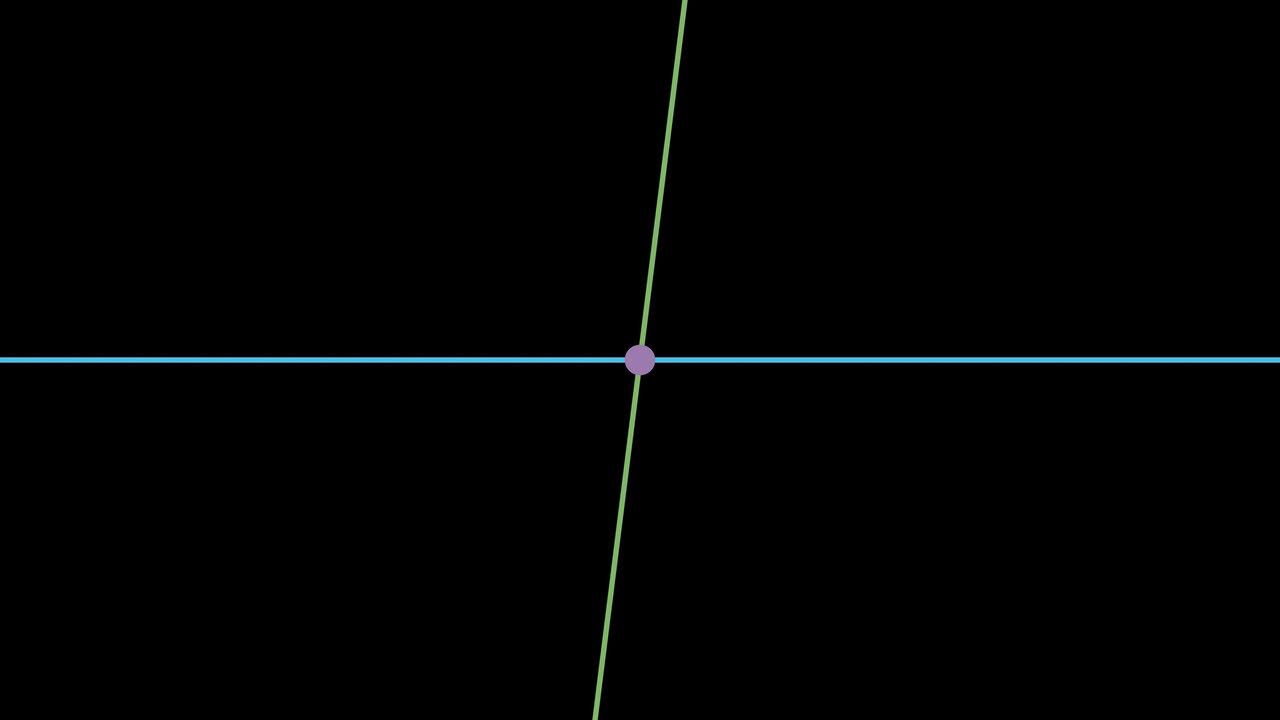
\includegraphics[width=0.33\linewidth]{assets/posedness1.jpg}\hfill
	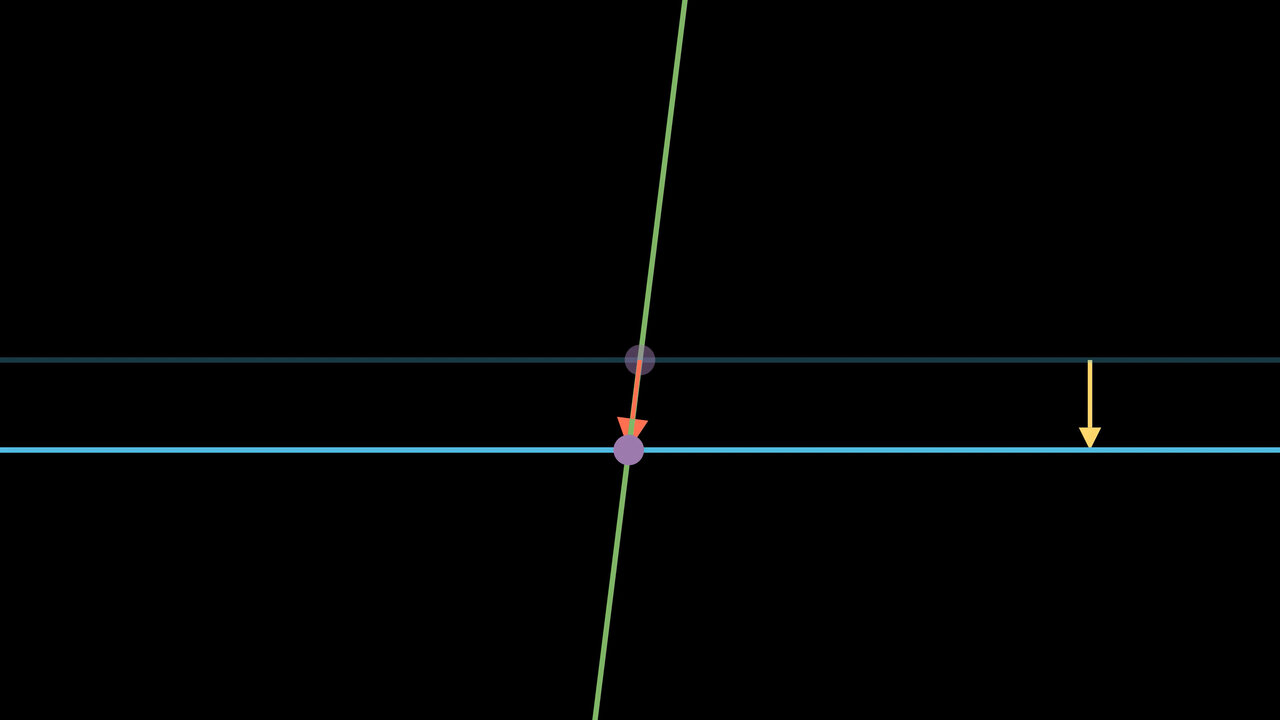
\includegraphics[width=0.33\linewidth]{assets/posedness2.jpg}\hfill
	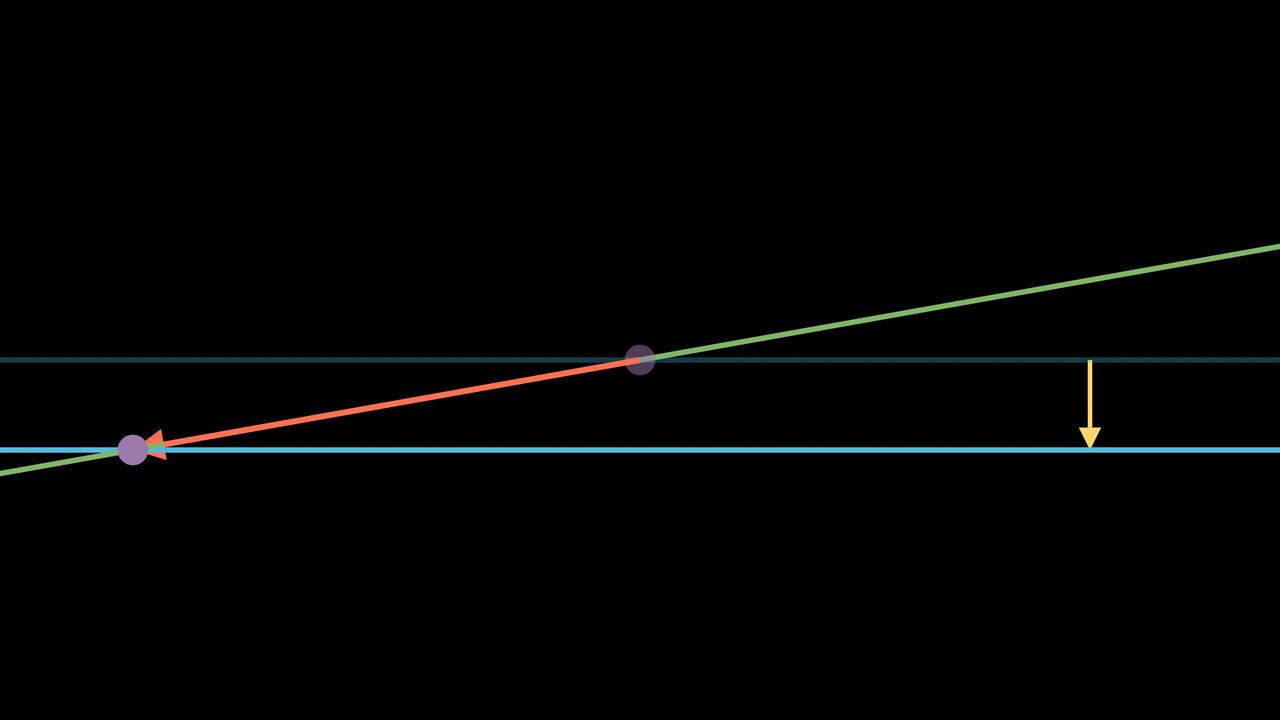
\includegraphics[width=0.33\linewidth]{assets/posedness3.jpg}
	\caption{Visualização geométrica do efeito do condicionamento sobre a solução de um sistema linear (bidimensional) cujo termo independente é perturbado.}
	\label{fig:posedness}
\end{figure}

\subsection*{Conteinerização do Ambiente de Programação}
A biblioteca Manim possui uma série de dependências em nível de sistema, como FFmpeg, OpenGL e alguma distribuição de \LaTeX{} (TeX Live ou MiKTeX, por exemplo).

Para não comprometer sistemas operacionais compartilhados entre múltiplos usuários (como os servidores de meu laboratório), aprendi o básico do software Docker, que permite encapsular tais dependências em um contêiner.

Tal encapsulamento, contudo, não foi trivial. Exigiu flexibilizar o isolamento do contêiner em três pontos:
\begin{enumerate}
    \item
    o acesso à GPU do sistema hospedeiro, de \textit{driver} variável (Mesa, para GPUs Intel e AMD, ou o \textit{driver} proprietário da NVIDIA);
    
    \item
    o acesso ao servidor de exibição, também variável (X11 ou Wayland);
    
    \item
    a execução com o ID do usuário que invoca o contêiner, de modo que os vídeos gerados possam ser acessados por ele sem privilégios de \texttt{root}.
\end{enumerate}

\subsection*{Confecção de Animações-Protótipo}
Em seguida, fiz correções à animação já existente e programei em Manim dois protótipos de cenas:
\begin{enumerate}
	\item um exibindo uma cerca na tela, que, posteriormente, guiado por meu orientador, transformei em um exemplo introdutório sobre condicionamento (vide a figura~\ref{fig:fence});
	\item outro destacando que os computadores possuem finitos dígitos para o armazenamento de números e, portanto, que erros são inevitáveis em contextos aplicados, assim como considerações sobre condicionamento (vide a figura~\ref{fig:computer}).
\end{enumerate}
\begin{figure}[htbp]
	\centering
	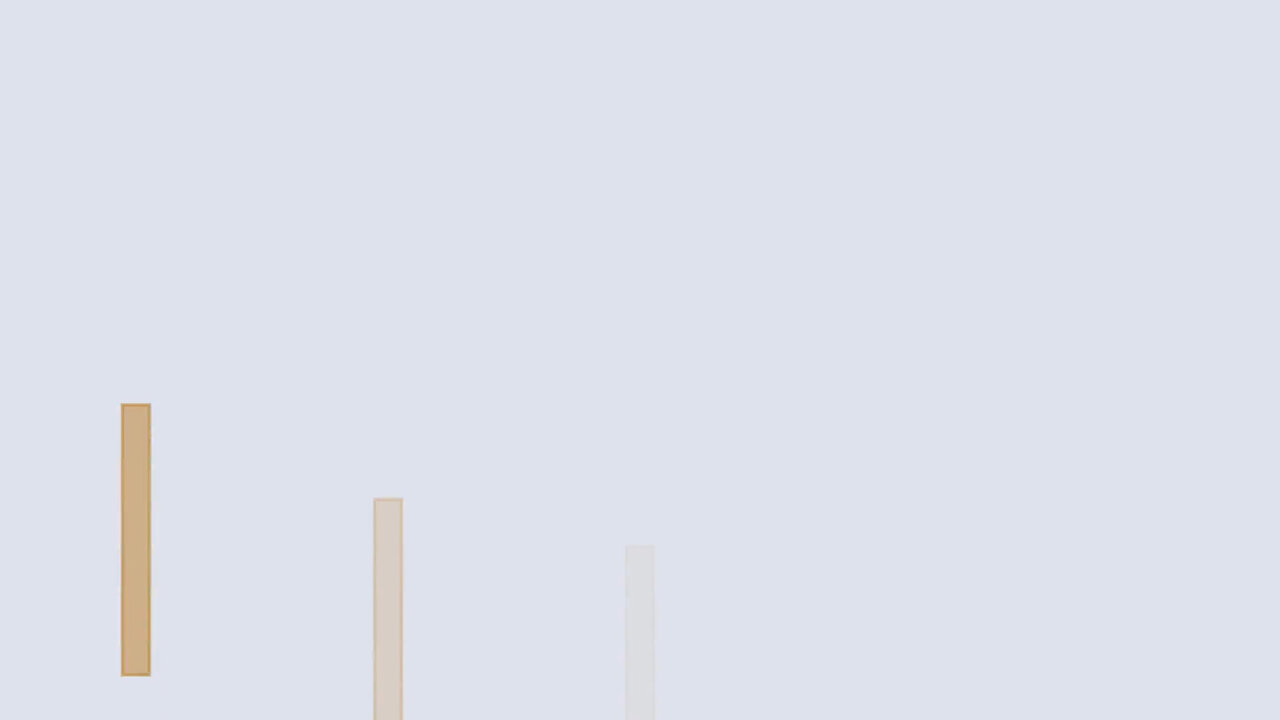
\includegraphics[width=0.325\linewidth]{assets/fence1.jpg}\hfill
	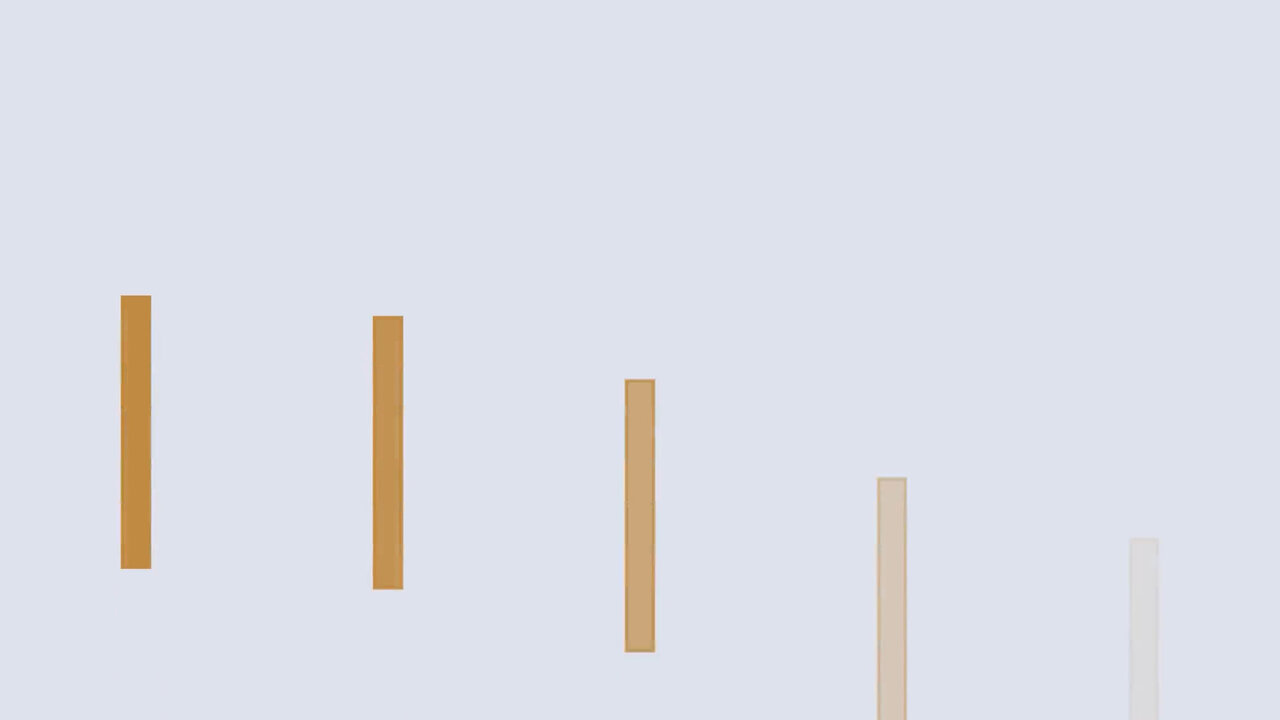
\includegraphics[width=0.325\linewidth]{assets/fence2.jpg}\hfill
	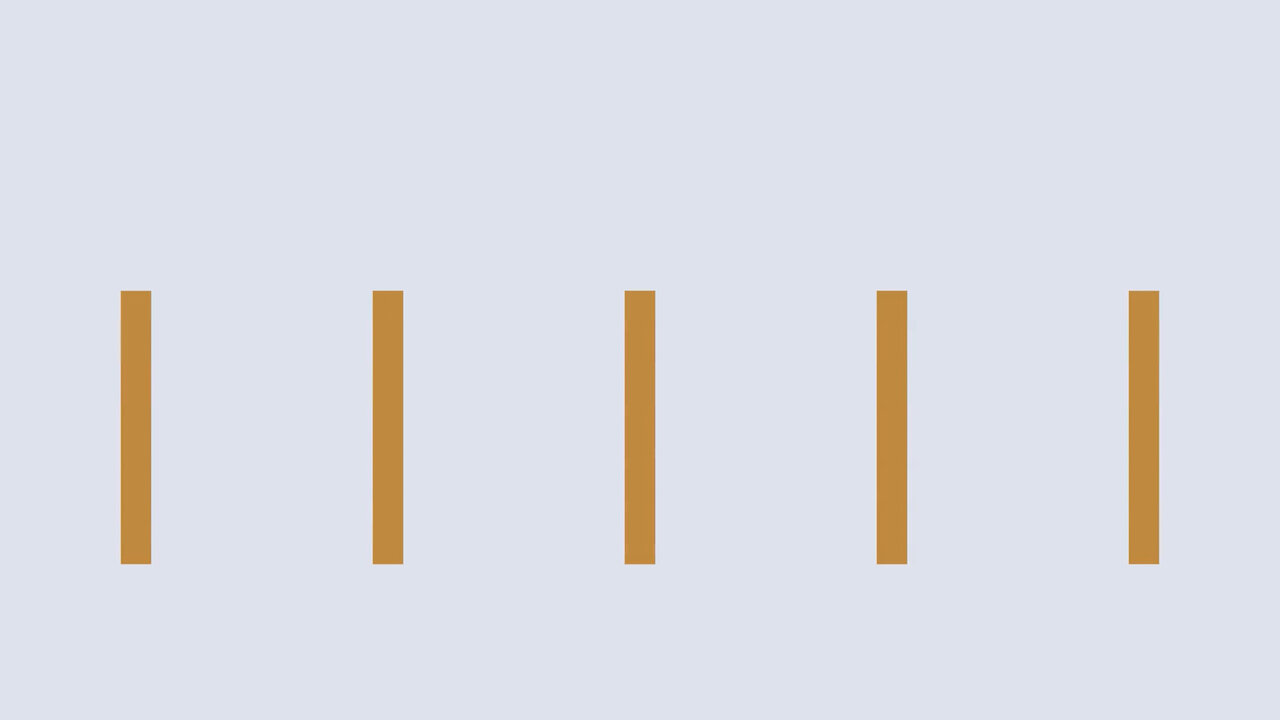
\includegraphics[width=0.325\linewidth]{assets/fence3.jpg}\\[0.5em]
	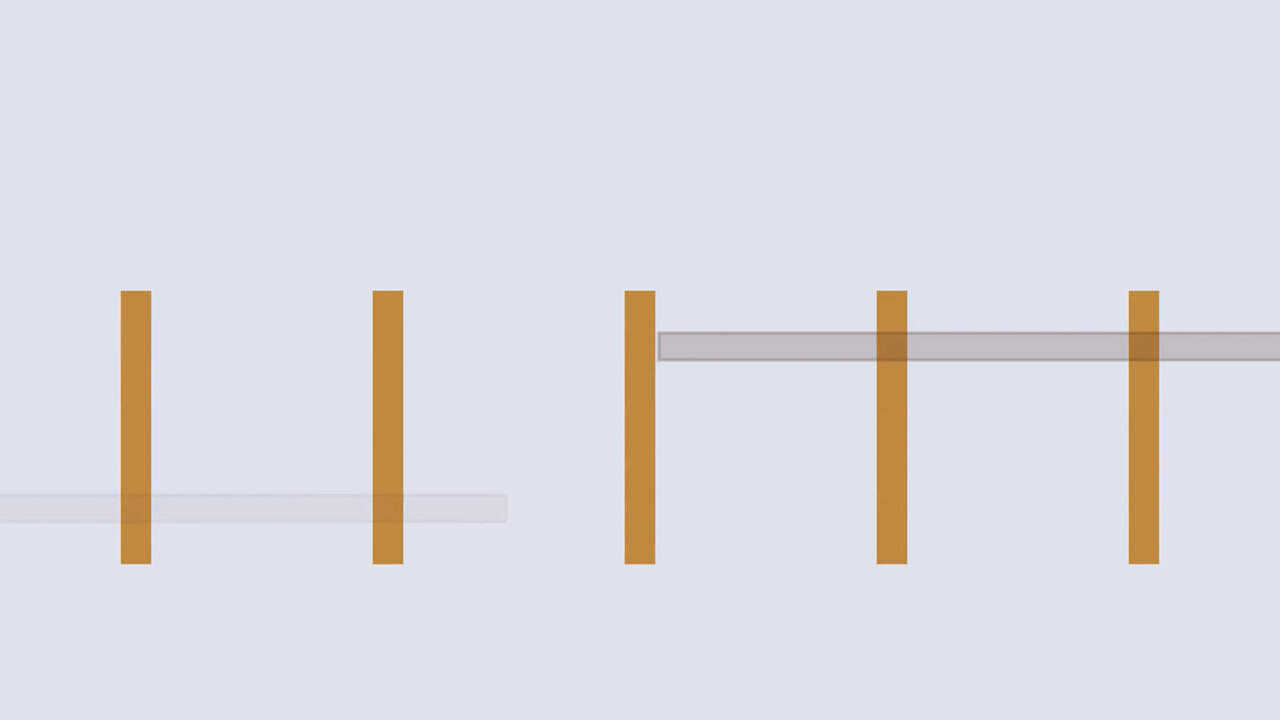
\includegraphics[width=0.325\linewidth]{assets/fence4.jpg}\hfill
	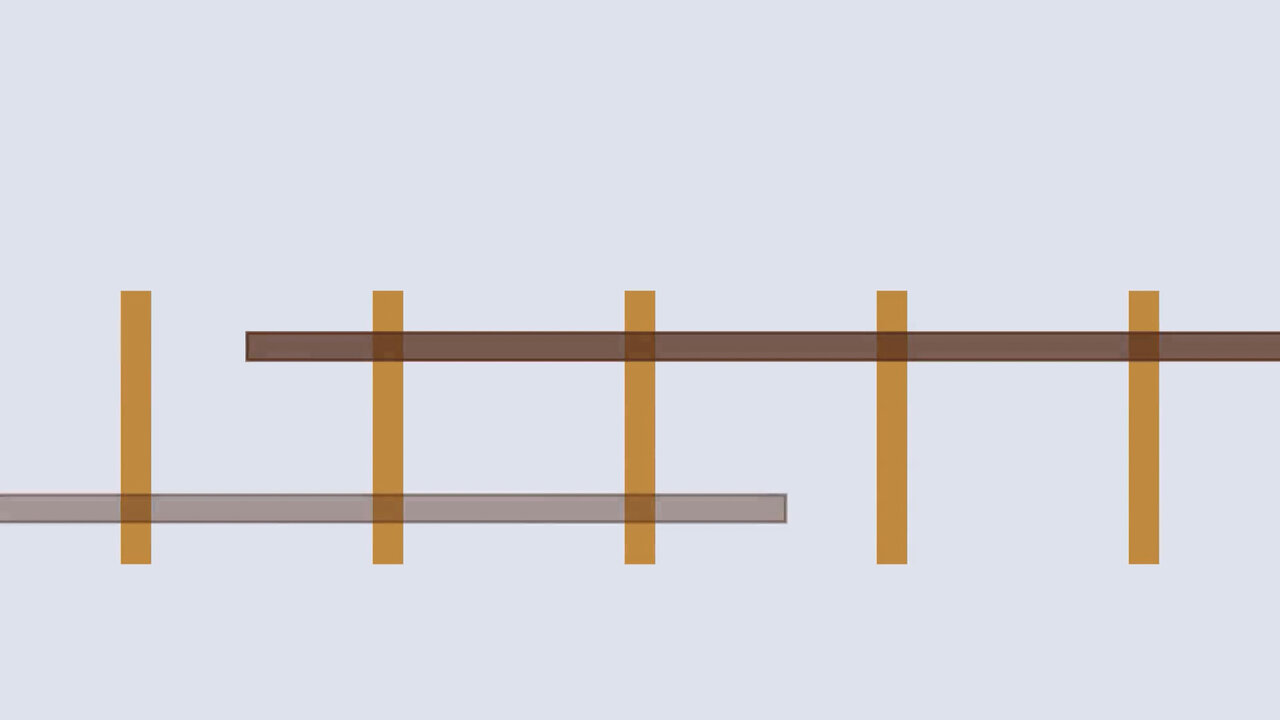
\includegraphics[width=0.325\linewidth]{assets/fence5.jpg}\hfill
	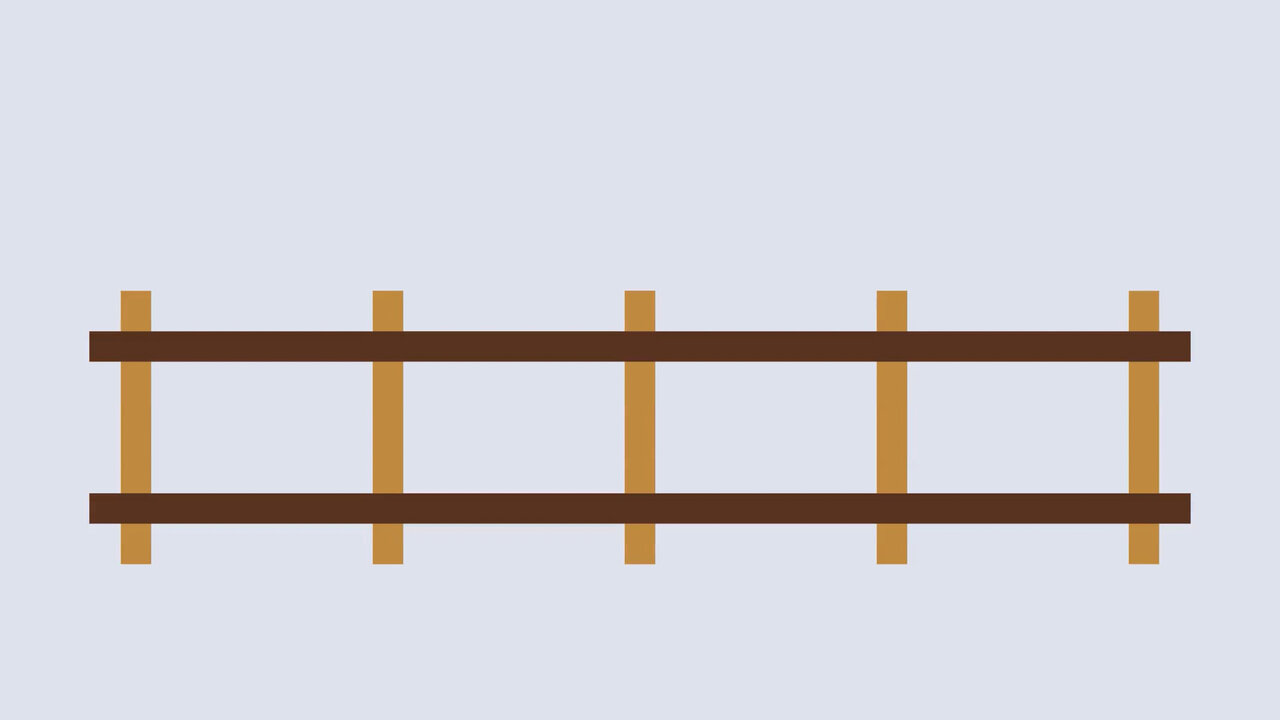
\includegraphics[width=0.325\linewidth]{assets/fence6.jpg}
	\caption{Visualização (com liberdades artísticas) da montagem de uma cerca.}
	\label{fig:fence}
\end{figure}
\begin{figure}[htbp]
	\centering
	
\includegraphics[width=0.325\linewidth]{assets/computer1.jpg}\hfill
	
\includegraphics[width=0.325\linewidth]{assets/computer2.jpg}\hfill
	
\includegraphics[width=0.325\linewidth]{assets/computer3.jpg}\\[0.5em]
	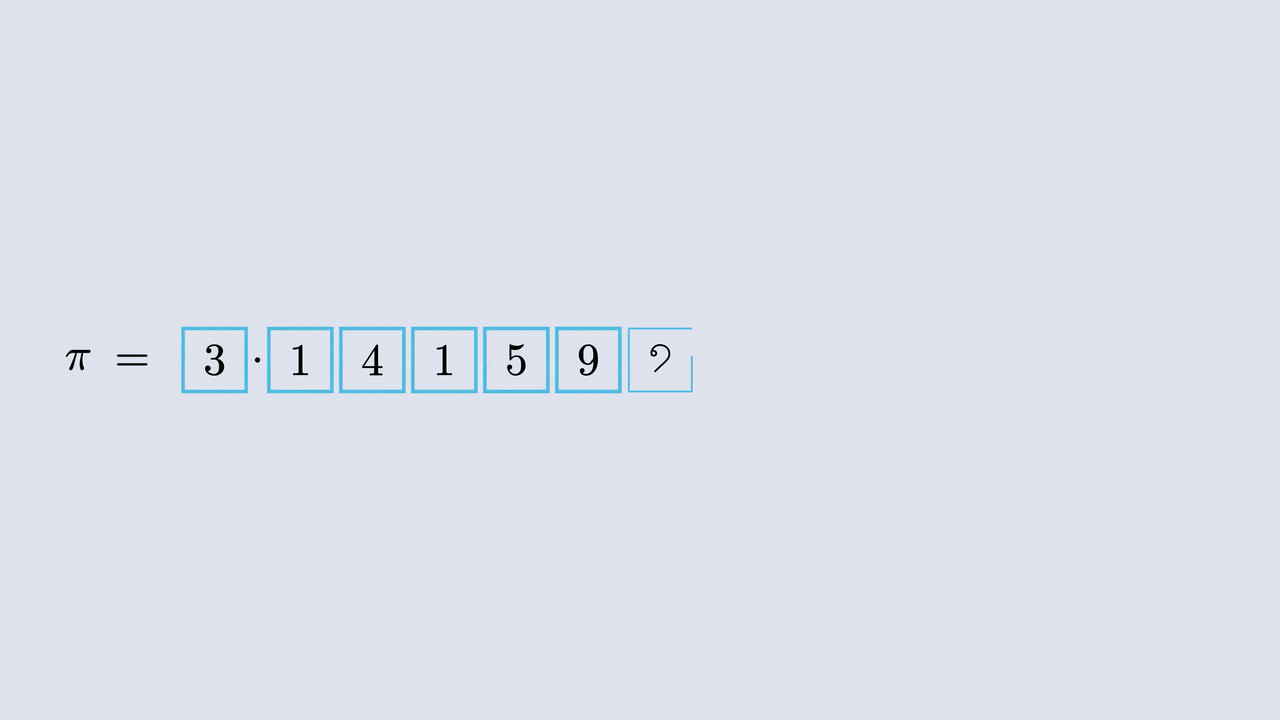
\includegraphics[width=0.325\linewidth]{assets/computer4.jpg}\hfill
	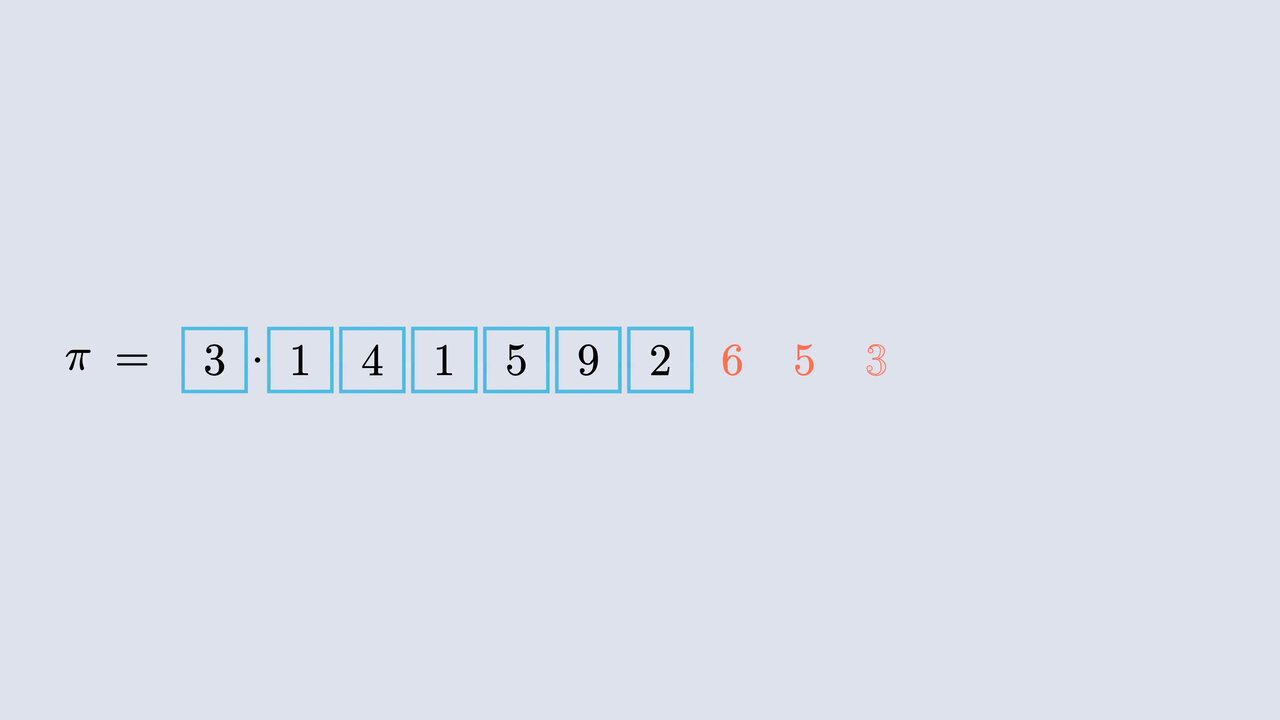
\includegraphics[width=0.325\linewidth]{assets/computer5.jpg}\hfill
	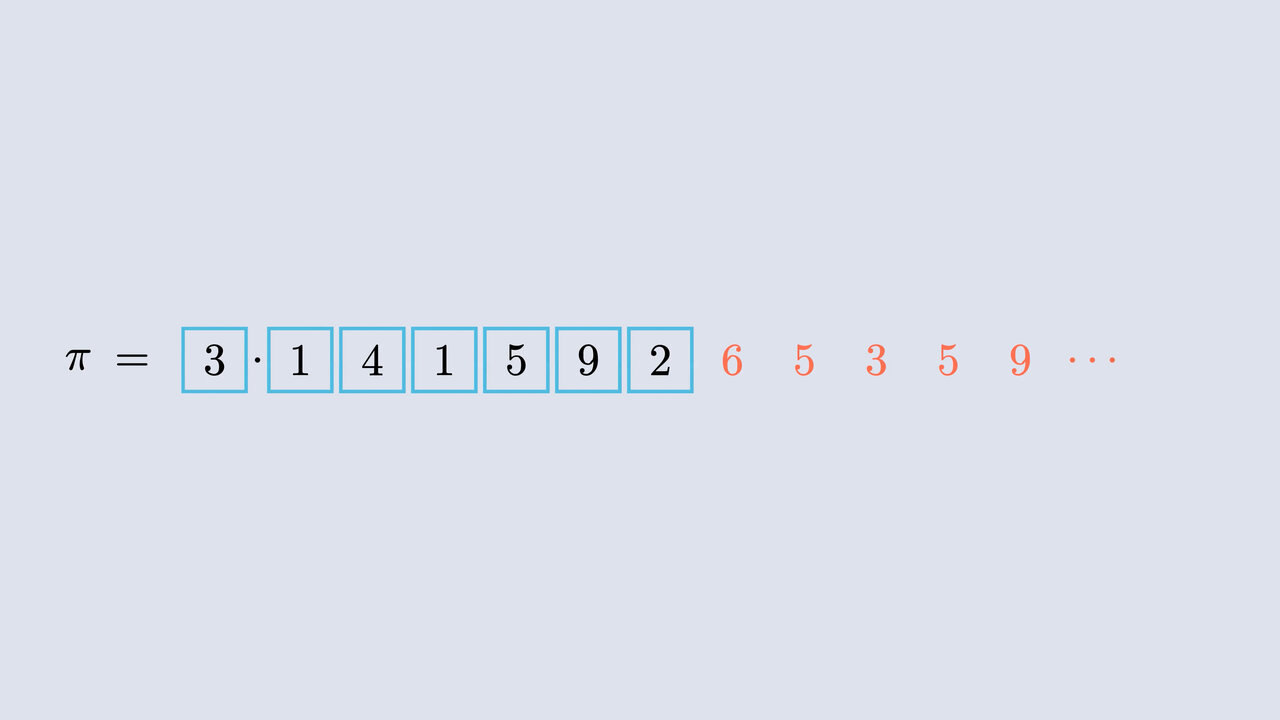
\includegraphics[width=0.325\linewidth]{assets/computer6.jpg}
	\caption{Imagens extraídas de uma animação comunicando que os computadores possuem finitos dígitos para o armazenamento de números e, portanto, que erros são inevitáveis em contextos aplicados, assim como considerações sobre condicionamento.}
	\label{fig:computer}
\end{figure}

\subsection*{Roteirização do Primeiro Vídeo}
Feitas as animações-protótipo, escrevi uma primeira versão do roteiro do primeiro vídeo para guiar-me na definição das próximas animações a serem confeccionadas.

Embora a maior parte dele tenha sido descartada, pois enfatizei conceitos demasiadamente elementares da matemática (como a definição de \emph{plano cartesiano}, por exemplo), tal roteiro ainda foi produtivo. Deixou-me claro o principal público-alvo de meu orientador e deste projeto: \emph{alunos no início de uma graduação em exatas, familiarizados com Cálculo Diferencial e Integral e Álgebra Linear}.

O motivo dessa escolha é simples: trata-se do público com a formação mínima para iniciar estudos na área de problemas inversos, mas que costuma desconhecê-la.

\subsection*{Animação sobre Sistemas Lineares}
Concomitantemente à roteirização do primeiro vídeo, elaborei uma animação do efeito geométrico de se ajustar coeficientes em uma equação linear (de duas variáveis).

A animação dos elementos textuais foi particularmente desafiadora. Como a largura e a altura de seus termos variam ao longo da animação, a simples inserção do texto em cada \textit{frame} leva a um efeito de trepidação, que distrai o espectador. Foi necessário ancorar cada termo separadamente e fazer bom uso de opções de formatação de \textit{strings} e de comandos \texttt{\textbackslash phantom\{\}} em \LaTeX{} para eliminá-lo.

Na figura~\ref{fig:linear}, é possível ver tanto os efeitos geométricos da variação de parâmetros quanto o bom alinhamento das equações algébricas correspondentes.
\begin{figure}[htbp]
	\centering
	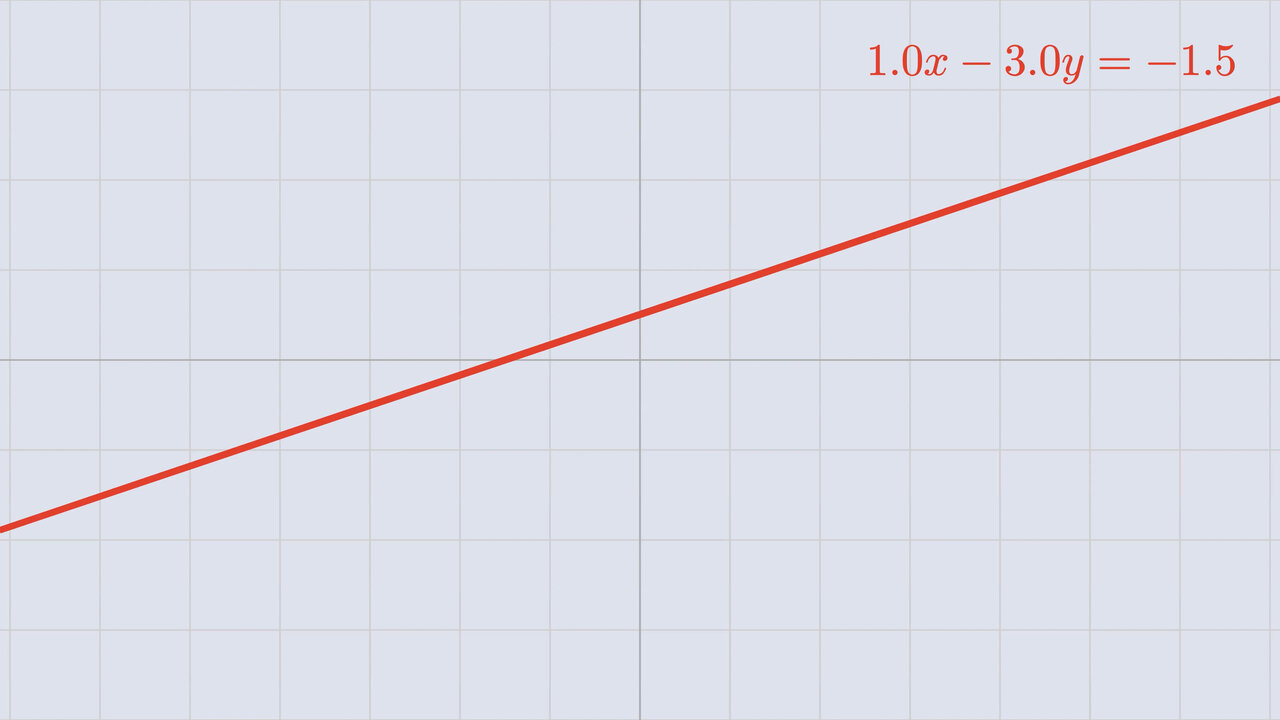
\includegraphics[width=0.325\linewidth]{assets/linear1.jpg}\hfill
	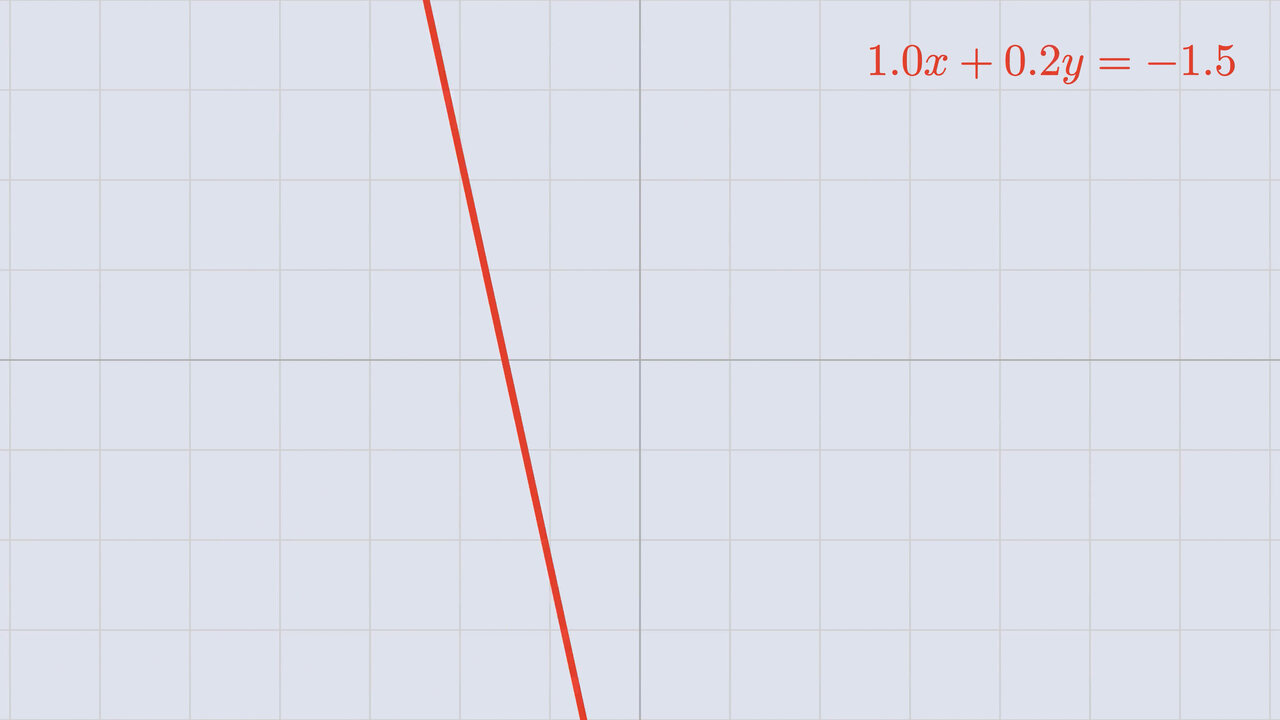
\includegraphics[width=0.325\linewidth]{assets/linear2.jpg}\hfill
	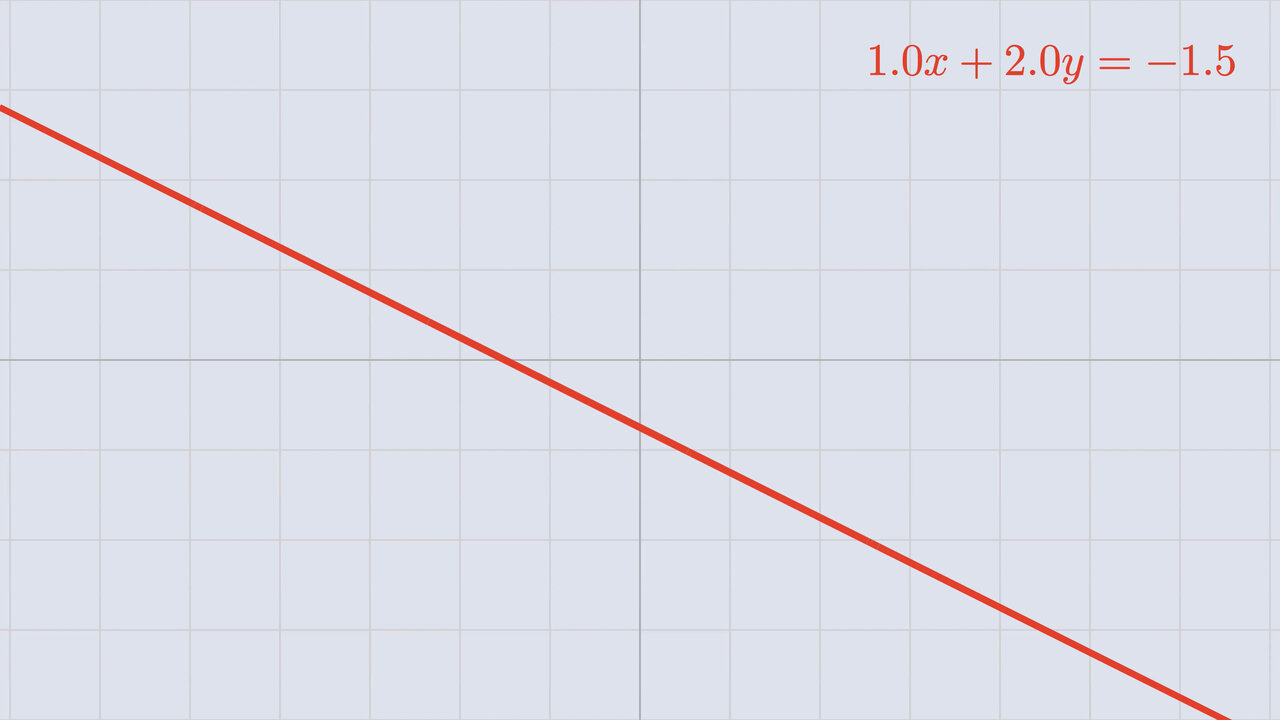
\includegraphics[width=0.325\linewidth]{assets/linear3.jpg}\\[0.5em]
	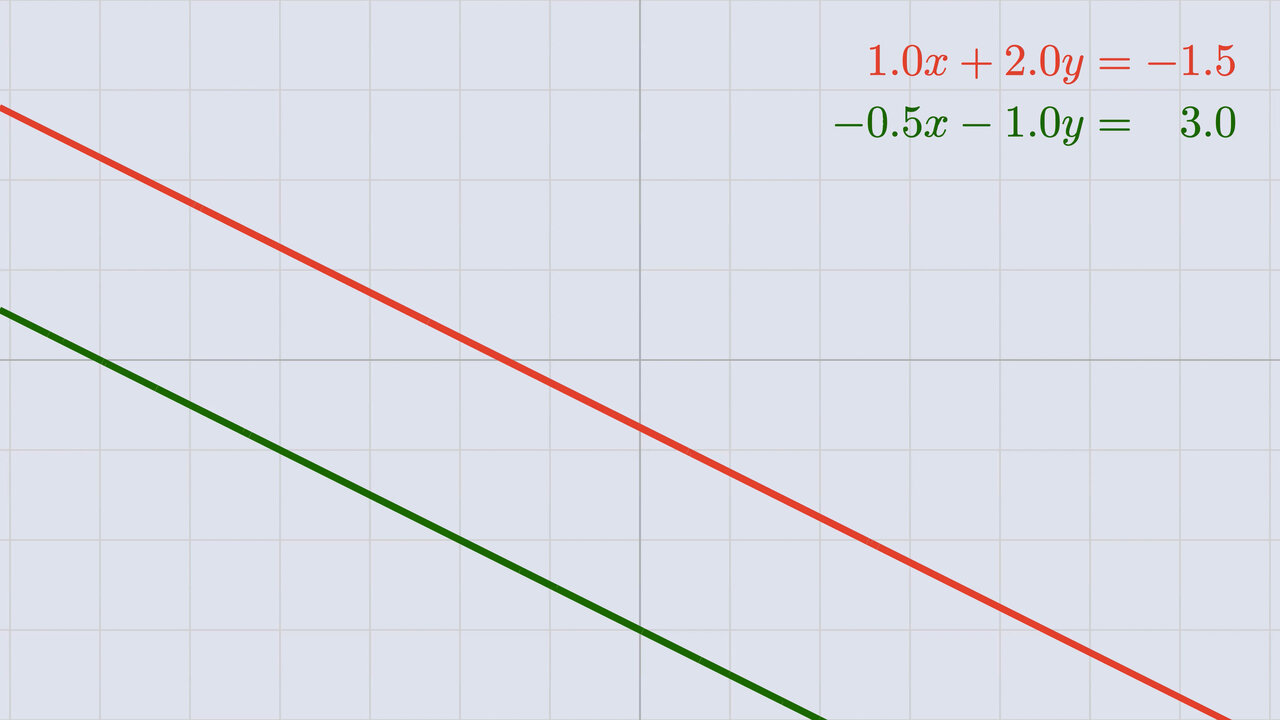
\includegraphics[width=0.325\linewidth]{assets/linear4.jpg}\hfill
	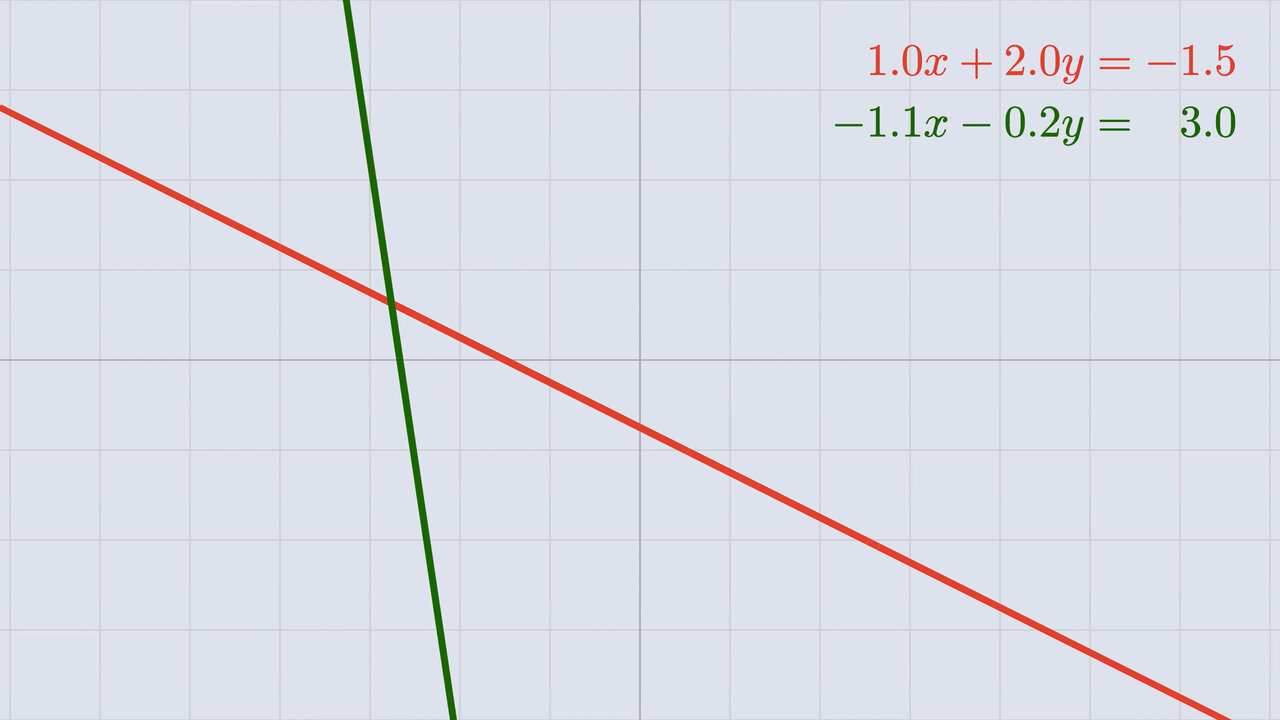
\includegraphics[width=0.325\linewidth]{assets/linear5.jpg}\hfill
	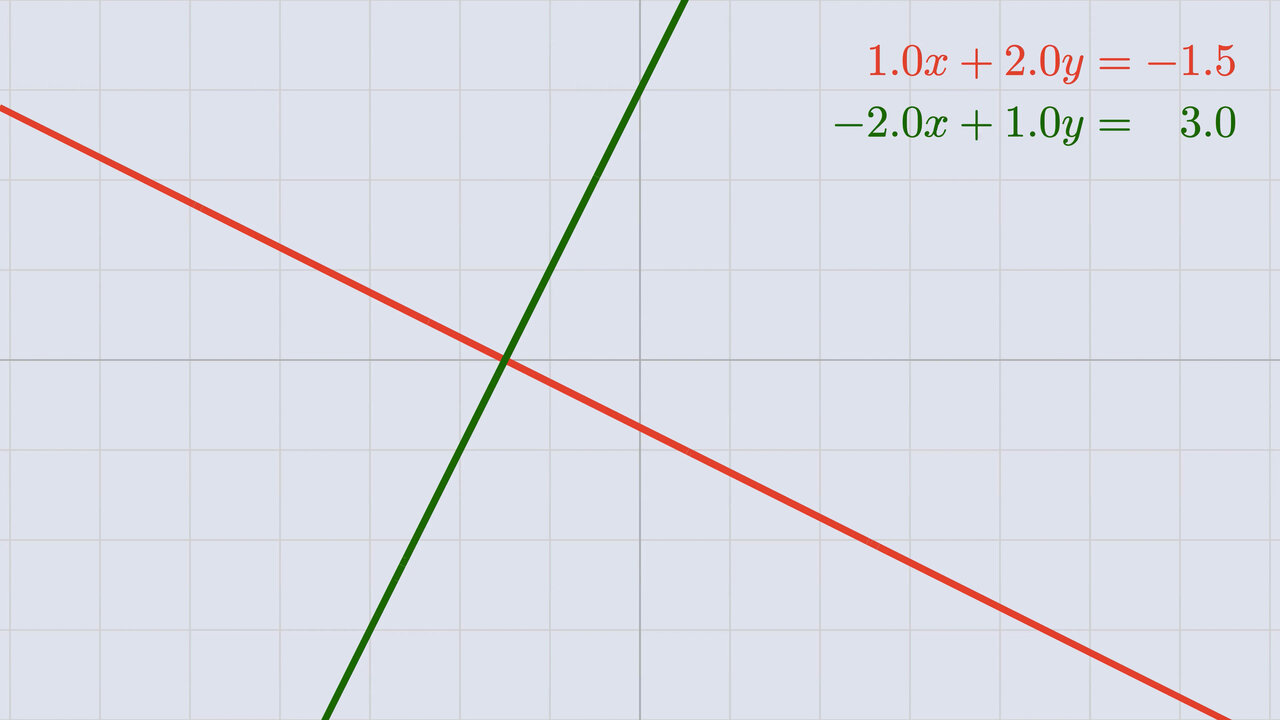
\includegraphics[width=0.325\linewidth]{assets/linear6.jpg}
	\caption{Efeito geométrico de se alterar os coeficientes de uma equação linear (de duas variáveis).}
	\label{fig:linear}
\end{figure}

\subsection*{Animação sobre Instalação de uma Cerca}
Em sequência, desenvolvi a animação da cerca. Primeiramente, fiz uma cena sobre a instalação de sua travessa. Se seus pontos de fixação são próximos de suas extremidades, pequenos erros afetam pouco sua orientação. À medida que os pontos de fixação se aproximam um do outro, tais erros podem ser amplificados a ponto de a instalação falhar, conforme visto na figura~\ref{fig:install}. Trata-se de um exemplo --- sugerido por meu orientador --- que transmite de forma muito intuitiva e acessível o conceito de condicionamento.
\begin{figure}[htbp]
	\centering
	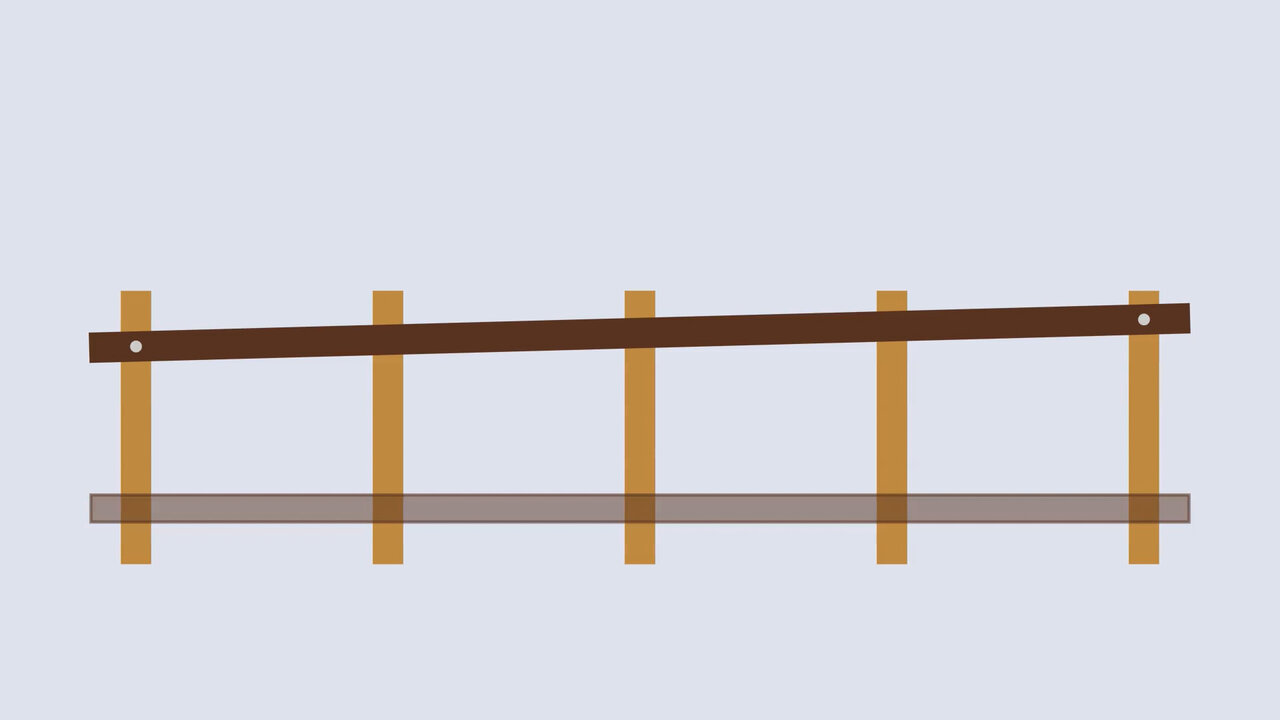
\includegraphics[width=0.325\linewidth]{assets/install1.jpg}\hfill
	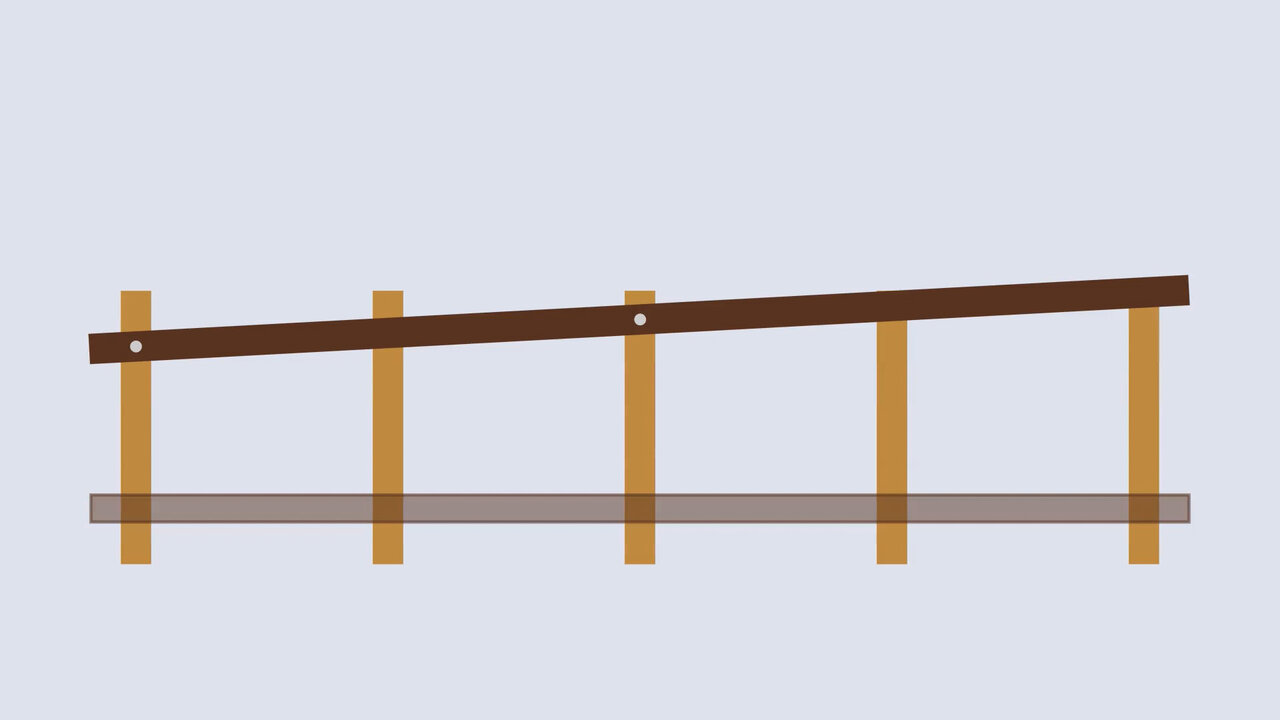
\includegraphics[width=0.325\linewidth]{assets/install2.jpg}\hfill
	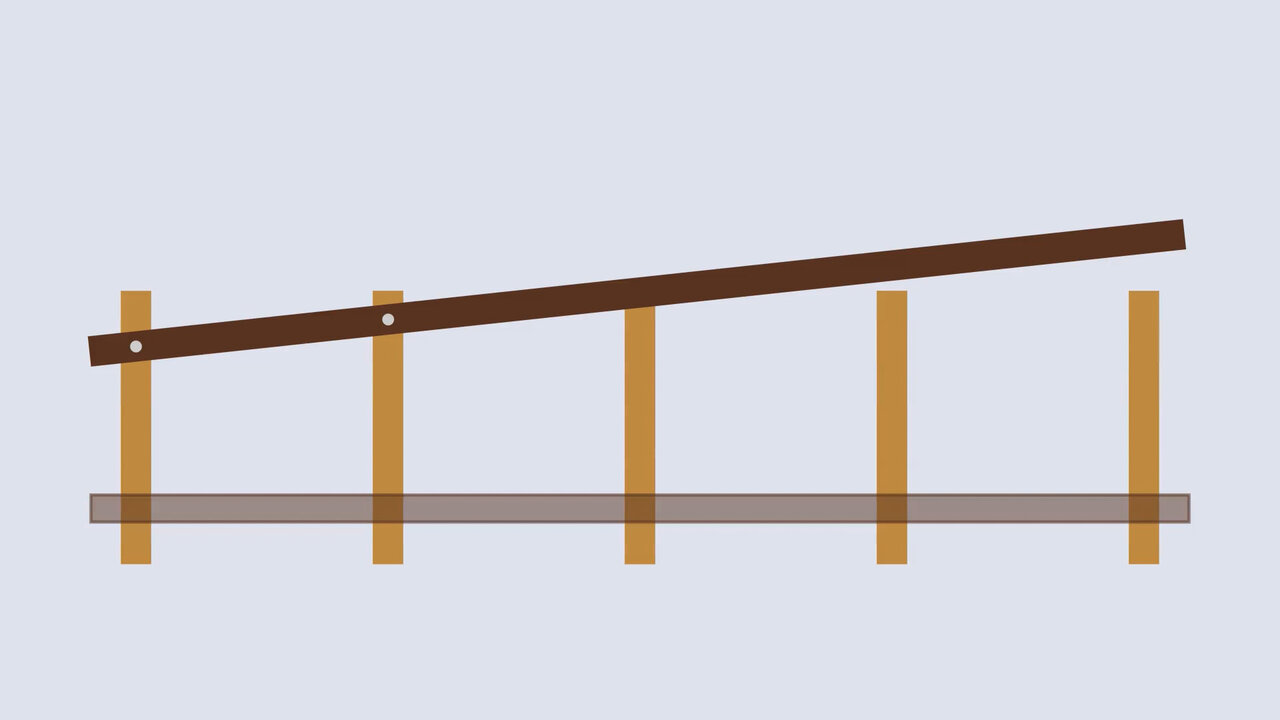
\includegraphics[width=0.325\linewidth]{assets/install3.jpg}
	\caption{Erro de instalação de uma travessa em função de seus pontos de fixação.}
	\label{fig:install}
\end{figure}

Ademais, modelei esse problema como um sistema linear simples, e confeccionei uma animação correspondente.

Elegendo um sistema de referência centrado no ponto em que o primeiro parafuso deve ser idealmente fixado, é possível parametrizar a travessa por uma equação de reta
\begin{equation*}
	y = ax + b,
\end{equation*}
em que $a$ é o coeficiente angular da travessa ($a = 0$ corresponde a uma travessa perfeitamente horizontal, como desejado) e $b$, o erro vertical em sua fixação (novamente, $b = 0$ é o valor ideal).

Por sua vez, sejam $y_1$ e $y_2$ os erros verticais cometidos em cada parafusação e $d$ a distância horizontal entre os dois parafusos. Por compatibilidade, as coordenadas dos parafusos --- $(0, y_1)$ e $(d, y_2)$ --- devem pertencer à reta que define a travessa, fornecendo as equações simultâneas
\begin{equation*}
	\begin{cases}
		y_1 = a0 + b \\
		y_2 = ad + b
	\end{cases}.
\end{equation*}
Ou, em forma matricial,
\begin{equation*}
	\begin{bmatrix}
		0 & 1 \\
		d & 1
	\end{bmatrix}
	\begin{bmatrix}
		a \\
		b
	\end{bmatrix}
	=
	\begin{bmatrix}
		y_1 \\
		y_2
	\end{bmatrix}.
\end{equation*}
Excertos da animação dessa modelagem podem ser vistos na figura~\ref{fig:modeling}.
\begin{figure}[htbp]
	\centering
	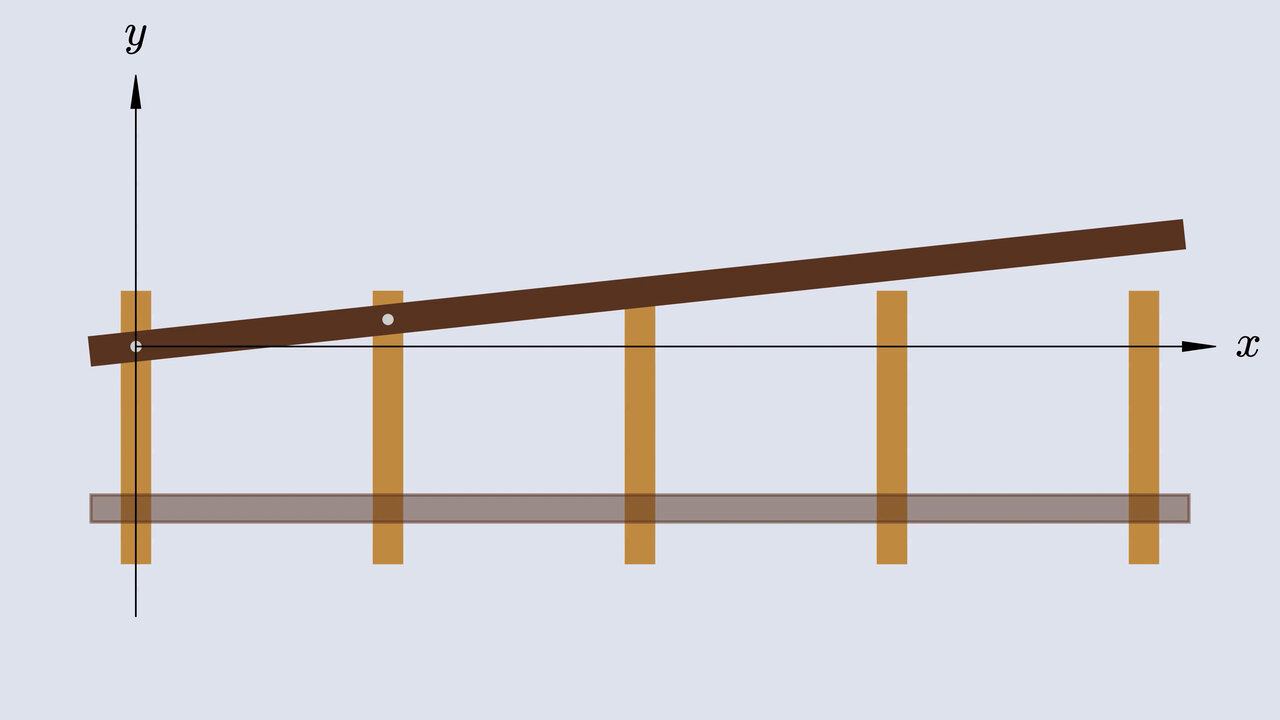
\includegraphics[width=0.325\linewidth]{assets/modeling1.jpg}\hfill
	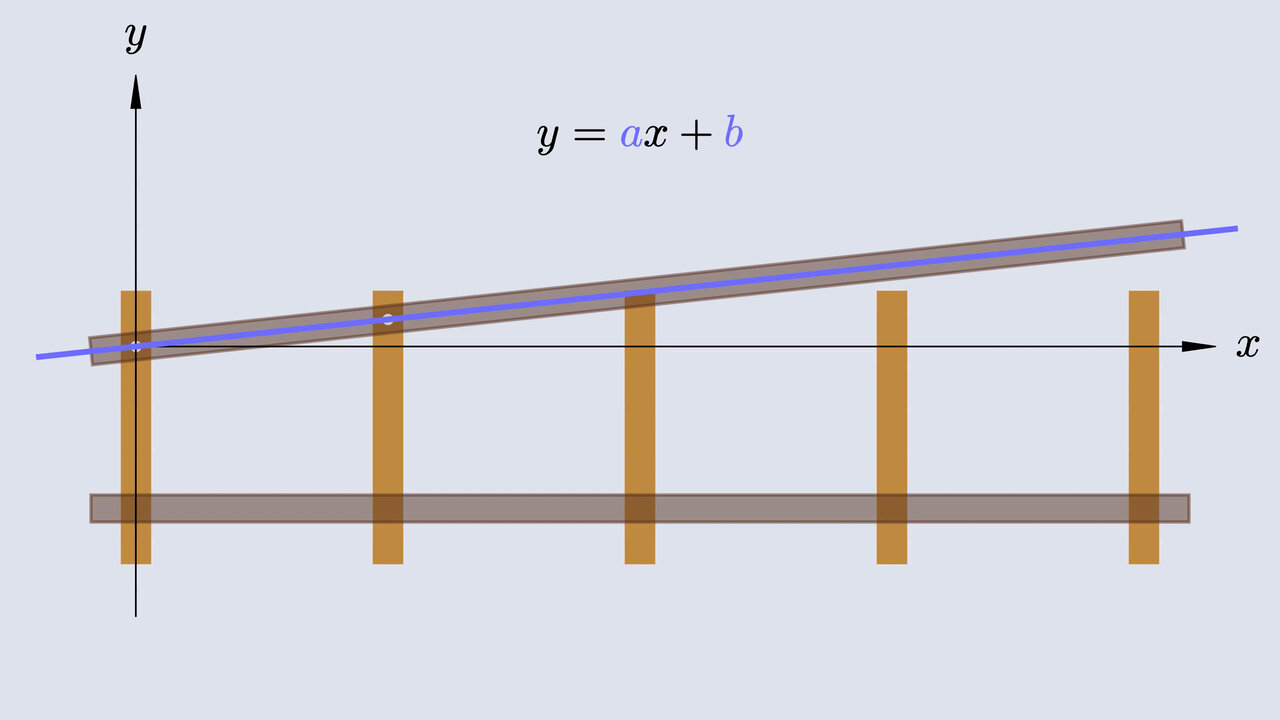
\includegraphics[width=0.325\linewidth]{assets/modeling2.jpg}\hfill
	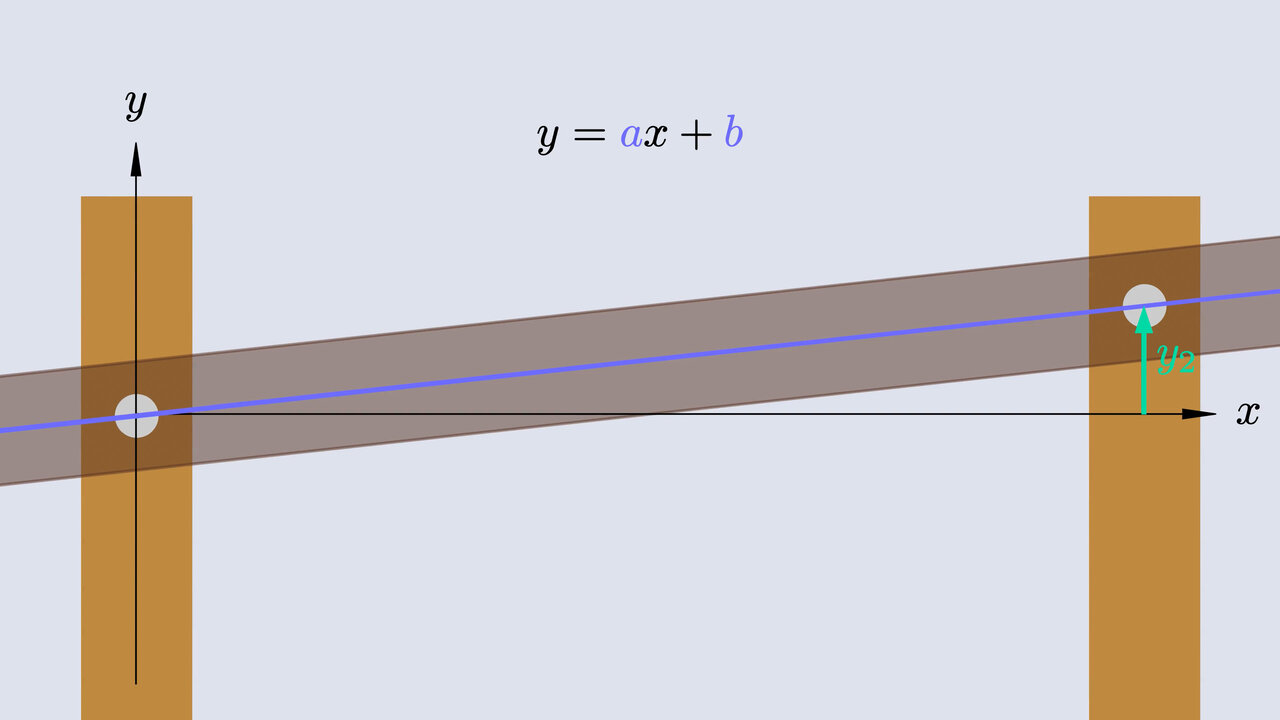
\includegraphics[width=0.325\linewidth]{assets/modeling3.jpg}\\[0.5em]
	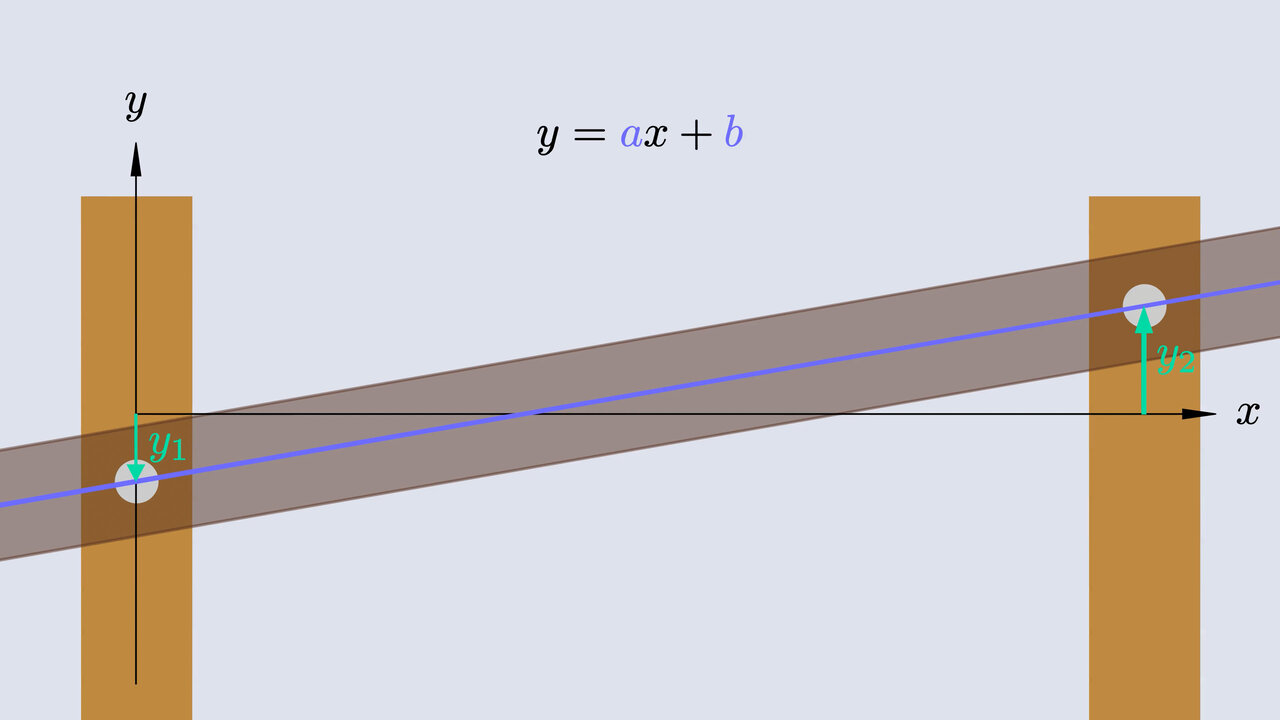
\includegraphics[width=0.325\linewidth]{assets/modeling4.jpg}\hfill
	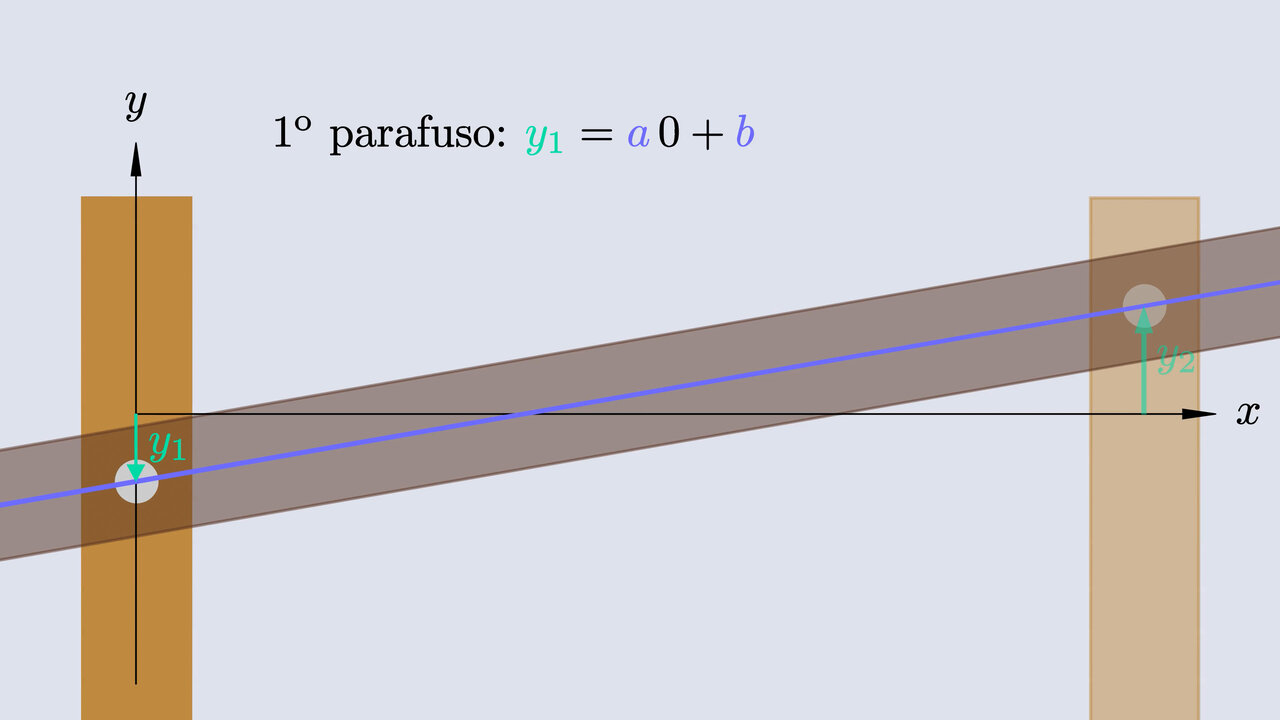
\includegraphics[width=0.325\linewidth]{assets/modeling5.jpg}\hfill
	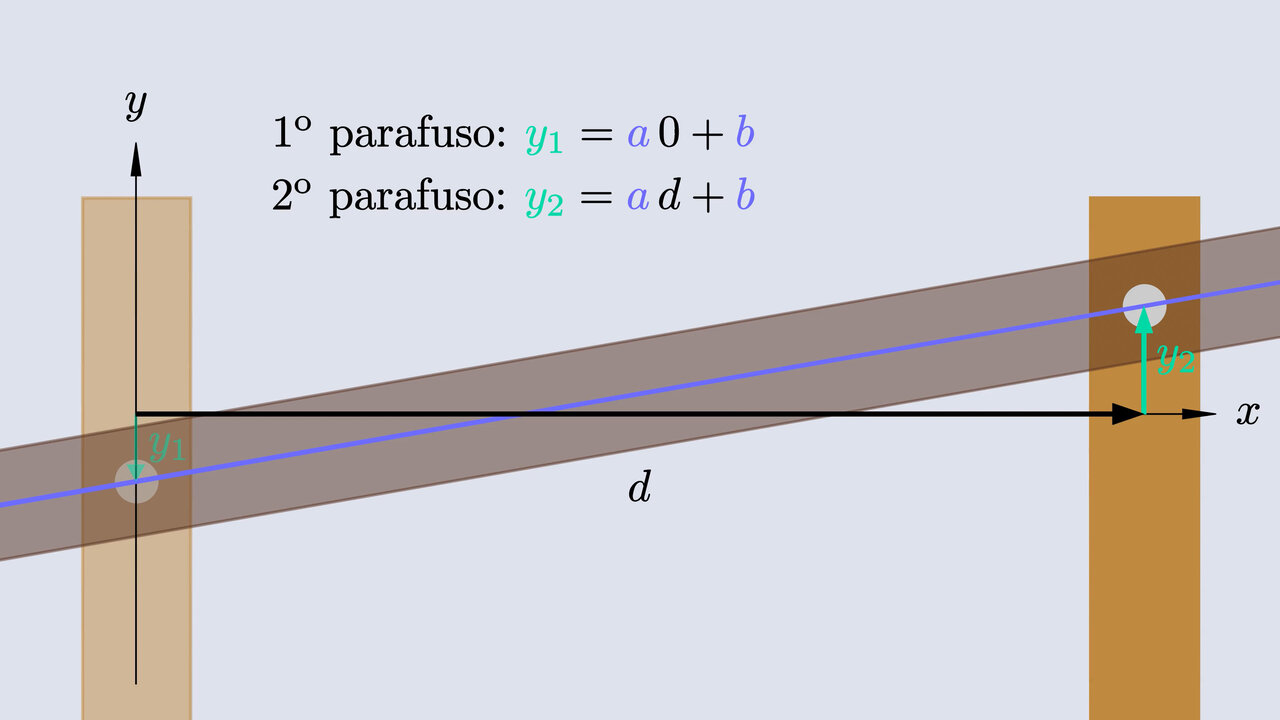
\includegraphics[width=0.325\linewidth]{assets/modeling6.jpg}\\[0.5em]
	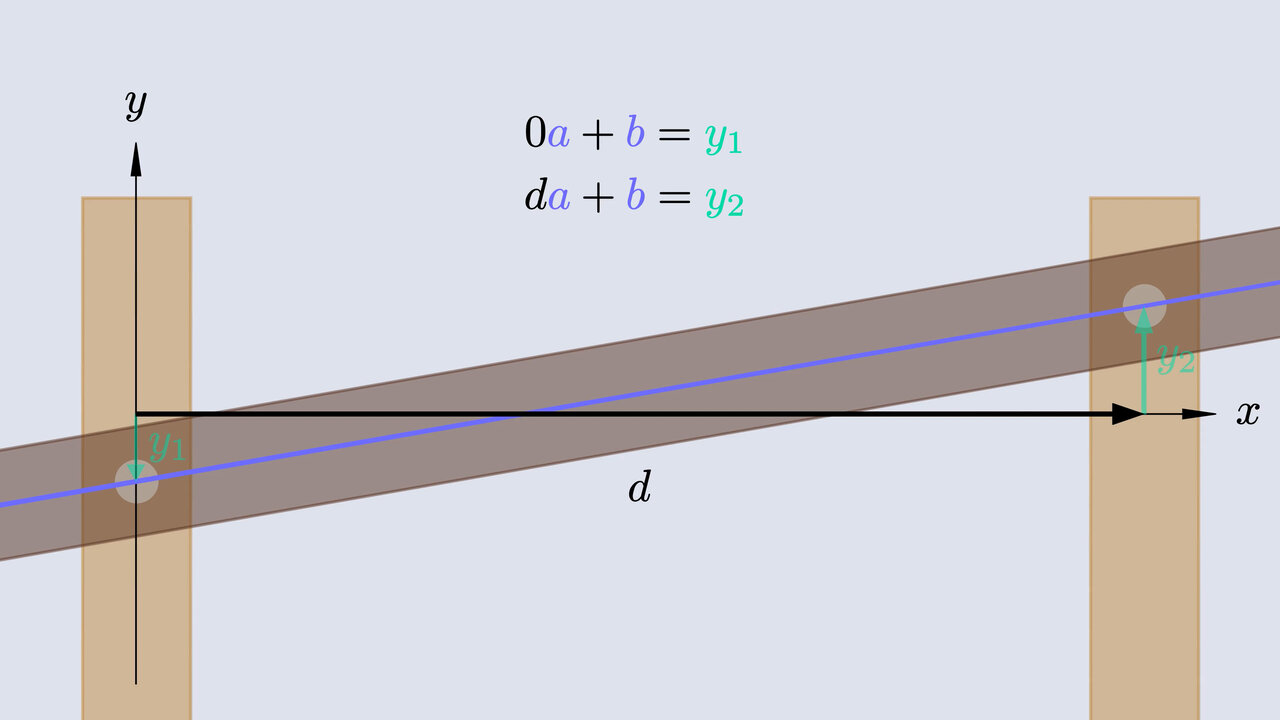
\includegraphics[width=0.325\linewidth]{assets/modeling7.jpg}\hfill
	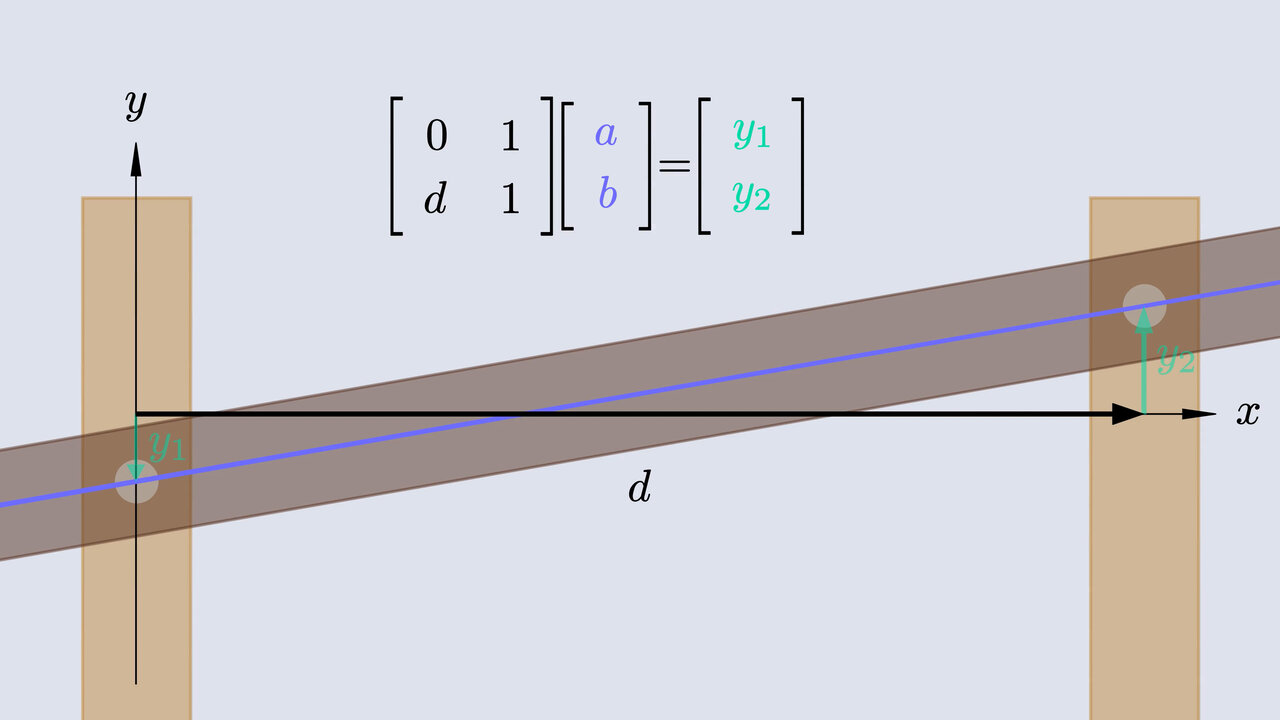
\includegraphics[width=0.325\linewidth]{assets/modeling8.jpg}\hfill
	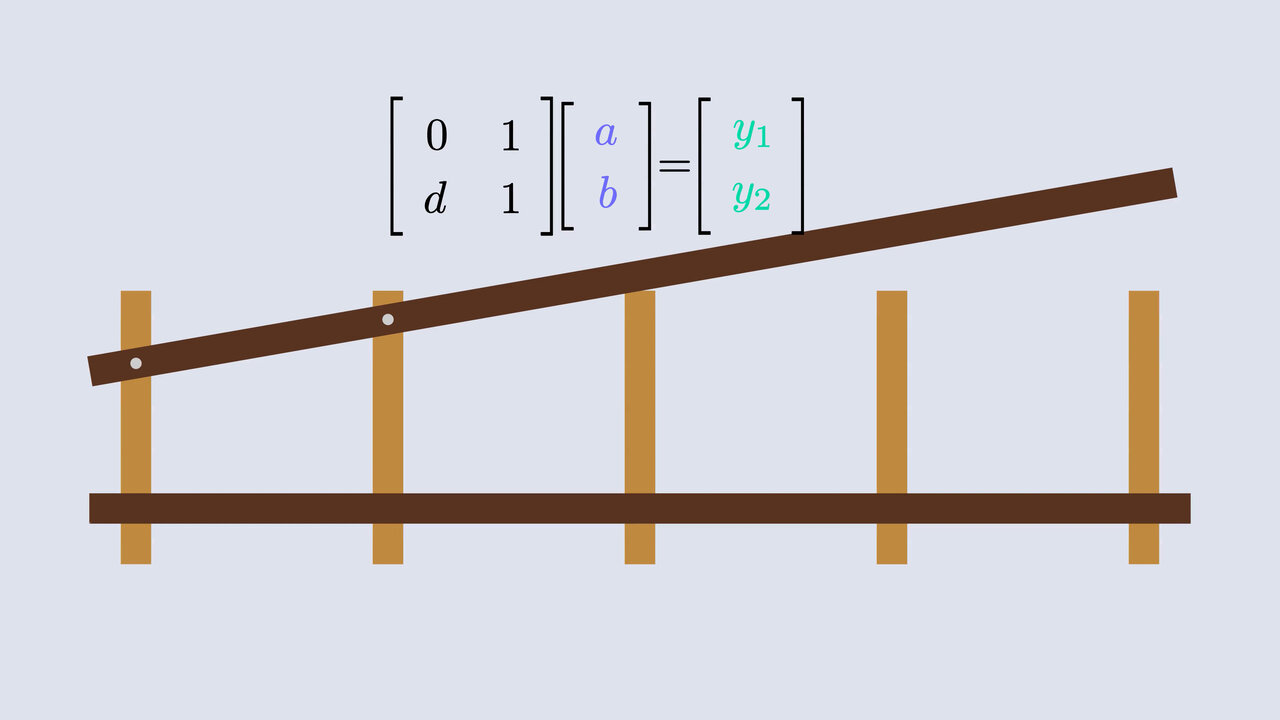
\includegraphics[width=0.325\linewidth]{assets/modeling9.jpg}
	\caption{Imagens extraídas de uma animação da modelagem de uma travessa parafusada a uma cerca como um sistema linear $2\times 2$.}
	\label{fig:modeling}
\end{figure}

Naturalmente, o próximo passo é animar a definição do número de condição $\kappa$ de uma matriz e o cálculo desse número para $M = \left[\begin{smallmatrix}0 & 1 \\ d & 1\end{smallmatrix}\right]$, em particular:
\begin{equation*}
	\kappa \coloneq \|M\|_2\|M^{-1}\|_2 = \frac{d^2 + 2 + \sqrt{d^4 + 4}}{2\lvert d\rvert}.
\end{equation*}
Concordando com a realidade física, temos que $\lim\limits_{d\to 0^+}\kappa = +\infty$.

\subsection*{Alinhamento com Bolsista de Jornalismo Científico}
Nos últimos dois meses, à medida que desenvolvia as animações relativas à cerca, passei a ter reuniões semanais não apenas com meu orientador, mas também com o bolsista de jornalismo científico. O estreitamento desse novo laço tem promovido progressos interessantes no projeto.

A título de exemplo, ao combinar minhas animações com gravações feitas por nosso orientador, o bolsista de jornalismo notou a carência de elementos visuais que guiassem a atenção do espectador. Por sugestão dele, incorporei efeitos de iluminação, mostrados na figura~\ref{fig:glow}.
\begin{figure}[htbp]
	\centering
	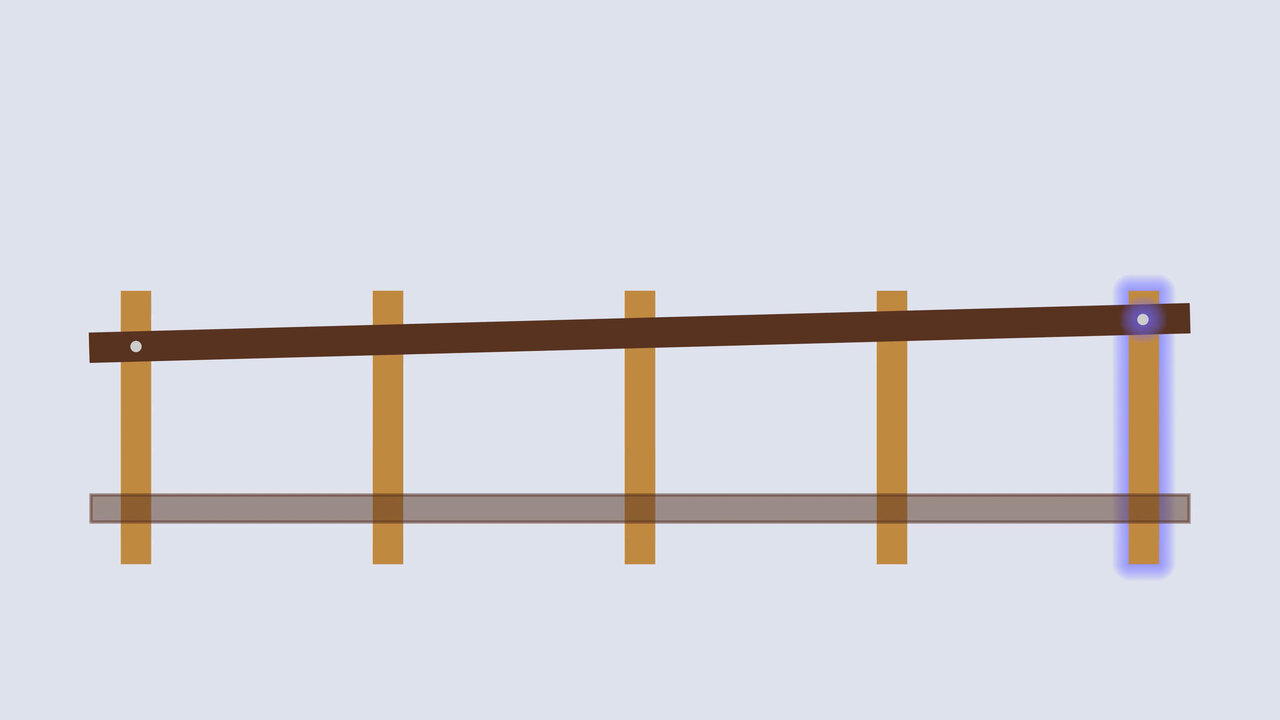
\includegraphics[width=0.325\linewidth]{assets/glow1.jpg}\hfill
	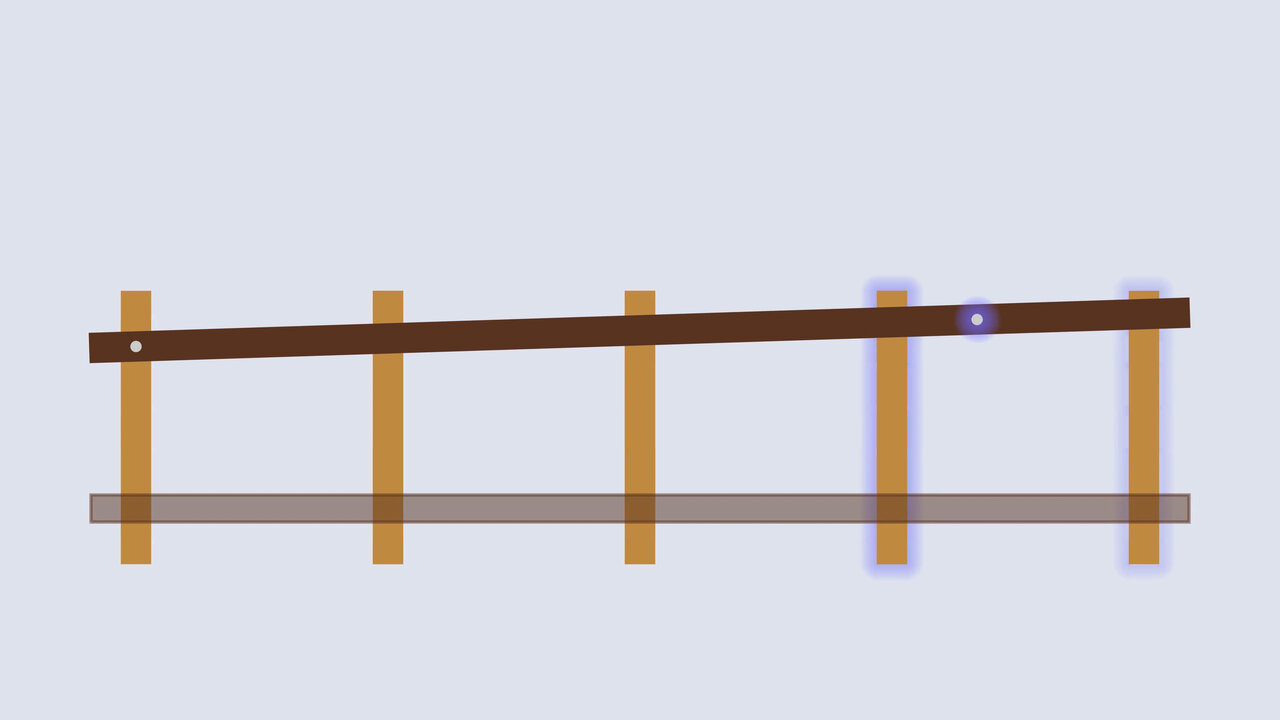
\includegraphics[width=0.325\linewidth]{assets/glow2.jpg}\hfill
	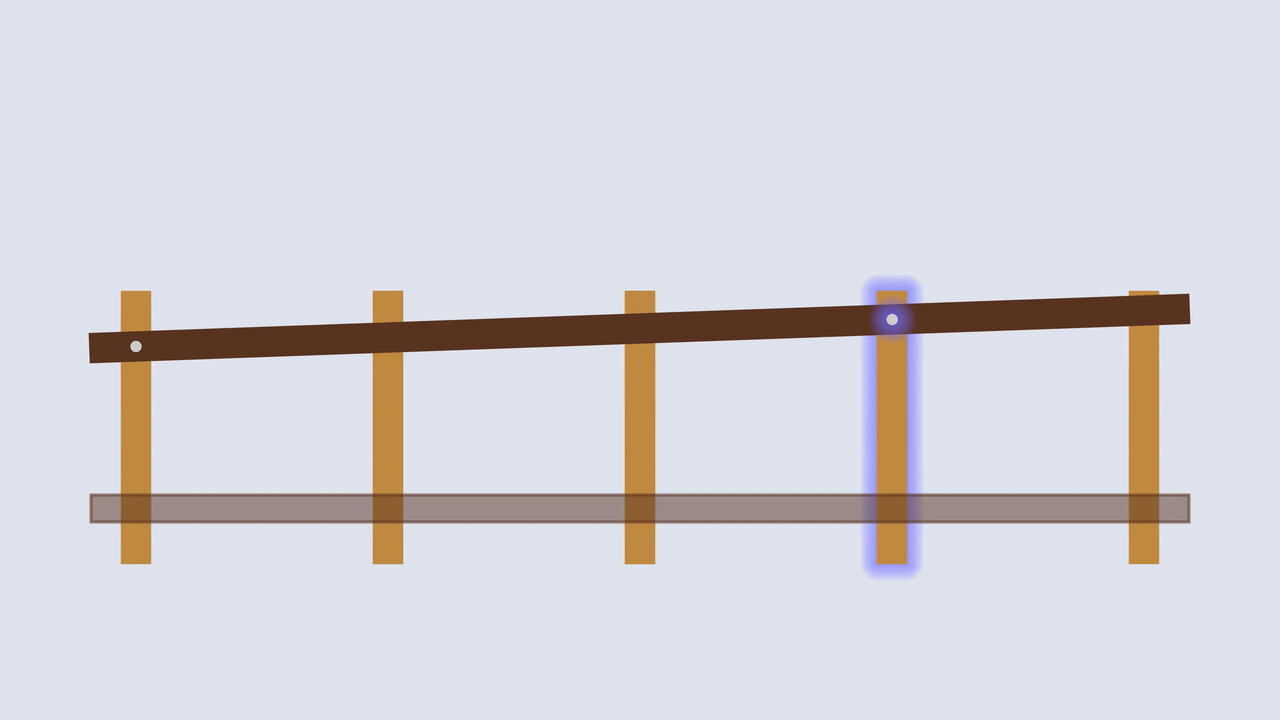
\includegraphics[width=0.325\linewidth]{assets/glow3.jpg}
	\caption{Efeito de iluminação para direcionar a atenção de um espectador.}
	\label{fig:glow}
\end{figure}

% 2.4) GESTÃO DE DADOS
\section*{Plano de Gestão de Dados}
Este projeto está gerando programas de computador. Em conformidade com o Plano de Gestão de Dados do projeto vinculado (2025/13357-1 --- Projeto de Pesquisa --- Regular), tais programas estão disponíveis em um repositório de código aberto:
\url{https://github.com/cody-setti/urp-manim-2026}.


% 3) PLANO DE ATIVIDADES
\section*{Plano de Atividades para o Próximo Período}
Concluir a confecção de uma série de vídeos introdutórios sobre otimização e problemas inversos, com ênfase na reconstrução de imagens.

% 4) EVENTOS
\section*{Participação em Eventos Científicos}
NADA A DECLARAR.


% 5) PUBLICAÇÕES
\section*{Publicações Resultantes da Bolsa}
NADA A DECLARAR.


% 7) TRABALHOS PREPARADOS
\section*{Trabalhos Preparados}
NADA A DECLARAR.


\begin{thebibliography}{9}
	\bibitem{trefethen}
	L.~N. Trefethen e D.~Bau~III.
	\textit{Numerical Linear Algebra}.
	SIAM, Philadelphia, 1997.
\end{thebibliography}

\end{document}

